\documentclass{article}

% if you need to pass options to natbib, use, e.g.:
\PassOptionsToPackage{numbers, compress}{natbib}
% before loading neurips_2026

% The authors should use one of these tracks.
% Before accepting by the NeurIPS conference, select one of the options below.
% 0. "default" for submission
% \usepackage{neurips_2026}
% the "default" option is equal to the "main" option, which is used for the Main Track with double-blind reviewing.
% 1. "main" option is used for the Main Track
%  \usepackage[main]{neurips_2026}
% 2. "position" option is used for the Position Paper Track
%  \usepackage[position]{neurips_2026}
% 3. "eandd" option is used for the Evaluations & Datasets Track
 % \usepackage[eandd]{neurips_2026}
% 4. "creativeai" option is used for the Creative AI Track
%  \usepackage[creativeai]{neurips_2026}
% 5. "sglblindworkshop" option is used for the Workshop with single-blind reviewing
 % \usepackage[sglblindworkshop]{neurips_2026}
% 6. "dblblindworkshop" option is used for the Workshop with double-blind reviewing
%  \usepackage[dblblindworkshop]{neurips_2026}

% After being accepted, the authors should add "final" behind the track to compile a camera-ready version.
% 1. Main Track
 % \usepackage[main, final]{neurips_2026}
% 2. Position Paper Track
%  \usepackage[position, final]{neurips_2026}
% 3. Evaluations & Datasets Track
 % \usepackage[eandd, final]{neurips_2026}
% 4. Creative AI Track
%  \usepackage[creativeai, final]{neurips_2026}
% 5. Workshop with single-blind reviewing
%  \usepackage[sglblindworkshop, final]{neurips_2026}
% 6. Workshop with double-blind reviewing
%  \usepackage[dblblindworkshop, final]{neurips_2026}
% Note. For the workshop paper template, both \title{} and \workshoptitle{} are required, with the former indicating the paper title shown in the title and the latter indicating the workshop title displayed in the footnote.
% For workshops (5., 6.), the authors should add the name of the workshop, "\workshoptitle" command is used to set the workshop title.
% \workshoptitle{WORKSHOP TITLE}

% "preprint" option is used for arXiv or other preprint submissions
\usepackage[preprint]{neurips_2026}

\usepackage{etoc}
\usepackage{tocloft}

\usepackage{amssymb}
\usepackage{booktabs}
\usepackage{wrapfig}
\usepackage{graphicx}
\usepackage{enumitem}
\usepackage[utf8]{inputenc} % allow utf-8 input
\usepackage[T1]{fontenc}    % use 8-bit T1 fonts
\usepackage{hyperref}       % hyperlinks
\usepackage{url}            % simple URL typesetting
\usepackage{booktabs}       % professional-quality tables
\usepackage{amsfonts}       % blackboard math symbols
\usepackage{nicefrac}       % compact symbols for 1/2, etc.
\usepackage{listings}       % for code listings
\usepackage{microtype}      % microtypography
\usepackage{xcolor}         % colors
\usepackage{amsmath} 
\usepackage{pifont}
\usepackage[table]{xcolor}
\usepackage{multirow}
\usepackage{booktabs}
\usepackage{graphicx}

  \usepackage[most]{tcolorbox}
  \usepackage{listings}
  \usepackage{xcolor}

  \definecolor{promptbg}{RGB}{248,249,251}
  \definecolor{promptframe}{RGB}{210,214,220}
  \definecolor{prompttitle}{RGB}{35,45,60}

  \lstdefinestyle{promptstyle}{
      basicstyle=\ttfamily\scriptsize,
      breaklines=true,
      breakatwhitespace=false,
      columns=fullflexible,
      keepspaces=true,
      showstringspaces=false,
      frame=none,
      xleftmargin=0pt,
      xrightmargin=0pt,
      aboveskip=2pt,
      belowskip=2pt
  }

  \newtcolorbox{promptbox}[1]{
      enhanced,
      breakable,
      colback=promptbg,
      colframe=promptframe,
      coltitle=prompttitle,
      fonttitle=\bfseries\small,
      title=#1,
      boxrule=0.5pt,
      arc=2pt,
      left=6pt,
      right=6pt,
      top=5pt,
      bottom=5pt,
      before skip=6pt,
      after skip=8pt
  }



\definecolor{best}{HTML}{C8E6C9}
\definecolor{best2}{HTML}{BBDEFB}

% Note. For the workshop paper template, both \title{} and \workshoptitle{} are required, with the former indicating the paper title shown in the title and the latter indicating the workshop title displayed in the footnote. 
\title{IndusAgent: Reinforcing Open-Vocabulary Industrial Anomaly Detection with Agentic Tools}

% Zhenlong Yuan, Rongbin Tan, Kejin Cui, Min Qiu, Fangfang Lin, Mengmeng Wang, Yi Wang, Zijian Song, Zhiyuan Wang, Jiyuan Wang, Yue Wang, Shuhan Song, Huawei Cao



% \author{
% \textbf{
% Zhenlong Yuan\textsuperscript{1 *} \quad
% Rongbin Tan\textsuperscript{1 *} \quad
% Kejin Cui\textsuperscript{2} \quad
% Min Qiu\textsuperscript{2} \quad
% Fangfang Lin\textsuperscript{3} \quad
% }
% \\[0.6em]
% \textbf{
% Mengmeng Wang\textsuperscript{4} \quad
% Yi Wang\textsuperscript{1} \quad
% Zijian Song\textsuperscript{5 \ensuremath{\ddagger}} \quad
% Zhiyuan Wang\textsuperscript{1} \quad
% Jiyuan Wang\textsuperscript{6} \quad
% }
% \\[0.6em]
% \textbf{
% Yue Wang\textsuperscript{7} \quad
% Shuhan Song\textsuperscript{1 8 \textsection}
% Huawei Cao\textsuperscript{1 8}
% }
% \\[1.0em]
% \textsuperscript{1} State Key Lab of Processors, Institute of Computing Technology, CAS \quad
% \\[0.6em]
% \textsuperscript{2} Independent Researcher \quad
% \textsuperscript{3} Santa Clara University \quad
% \textsuperscript{4} New York University \quad
% \\[0.6em]
% \textsuperscript{5} Sun Yat-sen University \quad 
% \textsuperscript{6} Nanyang Technological University \quad
% \textsuperscript{7} Stanford University \quad
% \\[0.6em]
% \textsuperscript{8} University of Chinese Academy of Sciences, Beijing, China
% \\[0.6em]
% \footnotesize
% \textsuperscript{*}~Equal contribution\quad
% \textsuperscript{\ensuremath{\ddagger}}~Project Lead\quad
% \textsuperscript{\textsection}~Corresponding Author
% }

\author{
\textbf{
Rongbin Tan\textsuperscript{1 9 *} \quad
Fangfang Lin\textsuperscript{2 *} \quad
Zhenlong Yuan\textsuperscript{3 * \ensuremath{\ddagger}} \quad
Min Qiu\textsuperscript{4} \quad
Kejin Cui\textsuperscript{4} \quad
}
\\[0.6em]
\textbf{
Mengmeng Wang\textsuperscript{5} \quad
Yi Wang\textsuperscript{1} \quad
Zijian Song\textsuperscript{6} \quad
Zhiyuan Wang\textsuperscript{4} \quad
Jiyuan Wang\textsuperscript{7} \quad
}
\\[0.6em]
\textbf{
Yue Wang\textsuperscript{8} \quad
Shuhan Song\textsuperscript{1 9 \textsection}
Huawei Cao\textsuperscript{1 9}
}
\\[1.0em]
\textsuperscript{1} State Key Lab of Processors, Institute of Computing Technology, CAS \quad
\\[0.6em]
\textsuperscript{2} Santa Clara University \quad
\textsuperscript{3} LongCat Team \quad
\textsuperscript{4} Independent Researcher \quad
\textsuperscript{5} New York University \quad
\\[0.6em]
\textsuperscript{6} Sun Yat-sen University \quad 
\textsuperscript{7} Nanyang Technological University \quad
\textsuperscript{8} Stanford University \quad
\\[0.6em]
\textsuperscript{9} University of Chinese Academy of Sciences, Beijing, China
\\[0.6em]
\footnotesize
\textsuperscript{*}~Equal contribution\quad
\textsuperscript{\ensuremath{\ddagger}}~Project Lead\quad
\textsuperscript{\textsection}~Corresponding Author
}


\begin{document}


\maketitle


\begin{abstract}
% Open-vocabulary industrial anomaly detection aims to identify unseen object categories and unpredictable defect types in real-world manufacturing scenarios. Although recent multimodal large language models provide strong zero-shot visual reasoning ability, they still struggle with fine-grained industrial inspection due to domain-misaligned reasoning, cross-modal hallucinations, and open-vocabulary generalization. To address these challenges, we propose \textbf{IndusAgent}, a tool-augmented agentic framework for open-vocabulary industrial anomaly detection. IndusAgent reformulates anomaly detection as an active visual reasoning process, where a vision-language model autonomously invokes external tools to gather high-resolution local evidence and priors. Specifically, we first construct a tool-integrated \textbf{Indus-CoT} dataset and perform Agentic Supervised Fine-Tuning to align the model with structured industrial diagnostic trajectories. We then introduce Agentic Reinforcement Learning based on GRPO, equipped with an efficiency-aware reward mechanism that jointly encourages diagnostic accuracy, localization quality, reasoning-format consistency, and judicious tool usage. 
% This design prevents indiscriminate tool invocation while enabling the model to actively resolve visual ambiguities. Experiments on five industrial anomaly detection benchmarks, including MVTec-AD, VisA, MPDD, DTD, and SDD, show that IndusAgent achieves strong open-vocabulary performance and robustness.


Multimodal large language models (MLLMs) have shown remarkable capability in bridging visual perception and textual reasoning, enabling zero-shot understanding across diverse industrial scenarios. However, their performance in open-vocabulary industrial anomaly detection (IAD) is often limited by domain-misaligned reasoning and hallucinated structural inferences. To address these challenges, we propose \textbf{IndusAgent}, a tool-augmented agentic framework for open-vocabulary IAD. Specifically, we first construct \textbf{Indus-CoT}, a structured dataset that integrates global visual observations, high-resolution local patches, and expert normalcy priors, providing supervision for fine-tuning the model on rigorous industrial inspection trajectories. Building on this, IndusAgent dynamically orchestrates a set of external tools, including dynamic region cropping, high-frequency feature enhancement, and prior retrieval, thus enabling the agent to actively resolve visual ambiguities and disentangle subtle anomalies. Furthermore, we introduce a gated reinforcement learning objective that jointly optimizes anomaly classification, localization accuracy, anomaly type reasoning, and efficient tool usage, ensuring that tool invocation occurs only when beneficial. Extensive evaluations on five industrial anomaly benchmarks, including MVTec-AD, VisA, MPDD, DTD, and SDD, demonstrate that IndusAgent achieves state-of-the-art zero-shot performance among all existing methods, validating our robustness and generalization capacity.

\end{abstract}

\section{Introduction}
\begin{figure} [h]
  \centering
  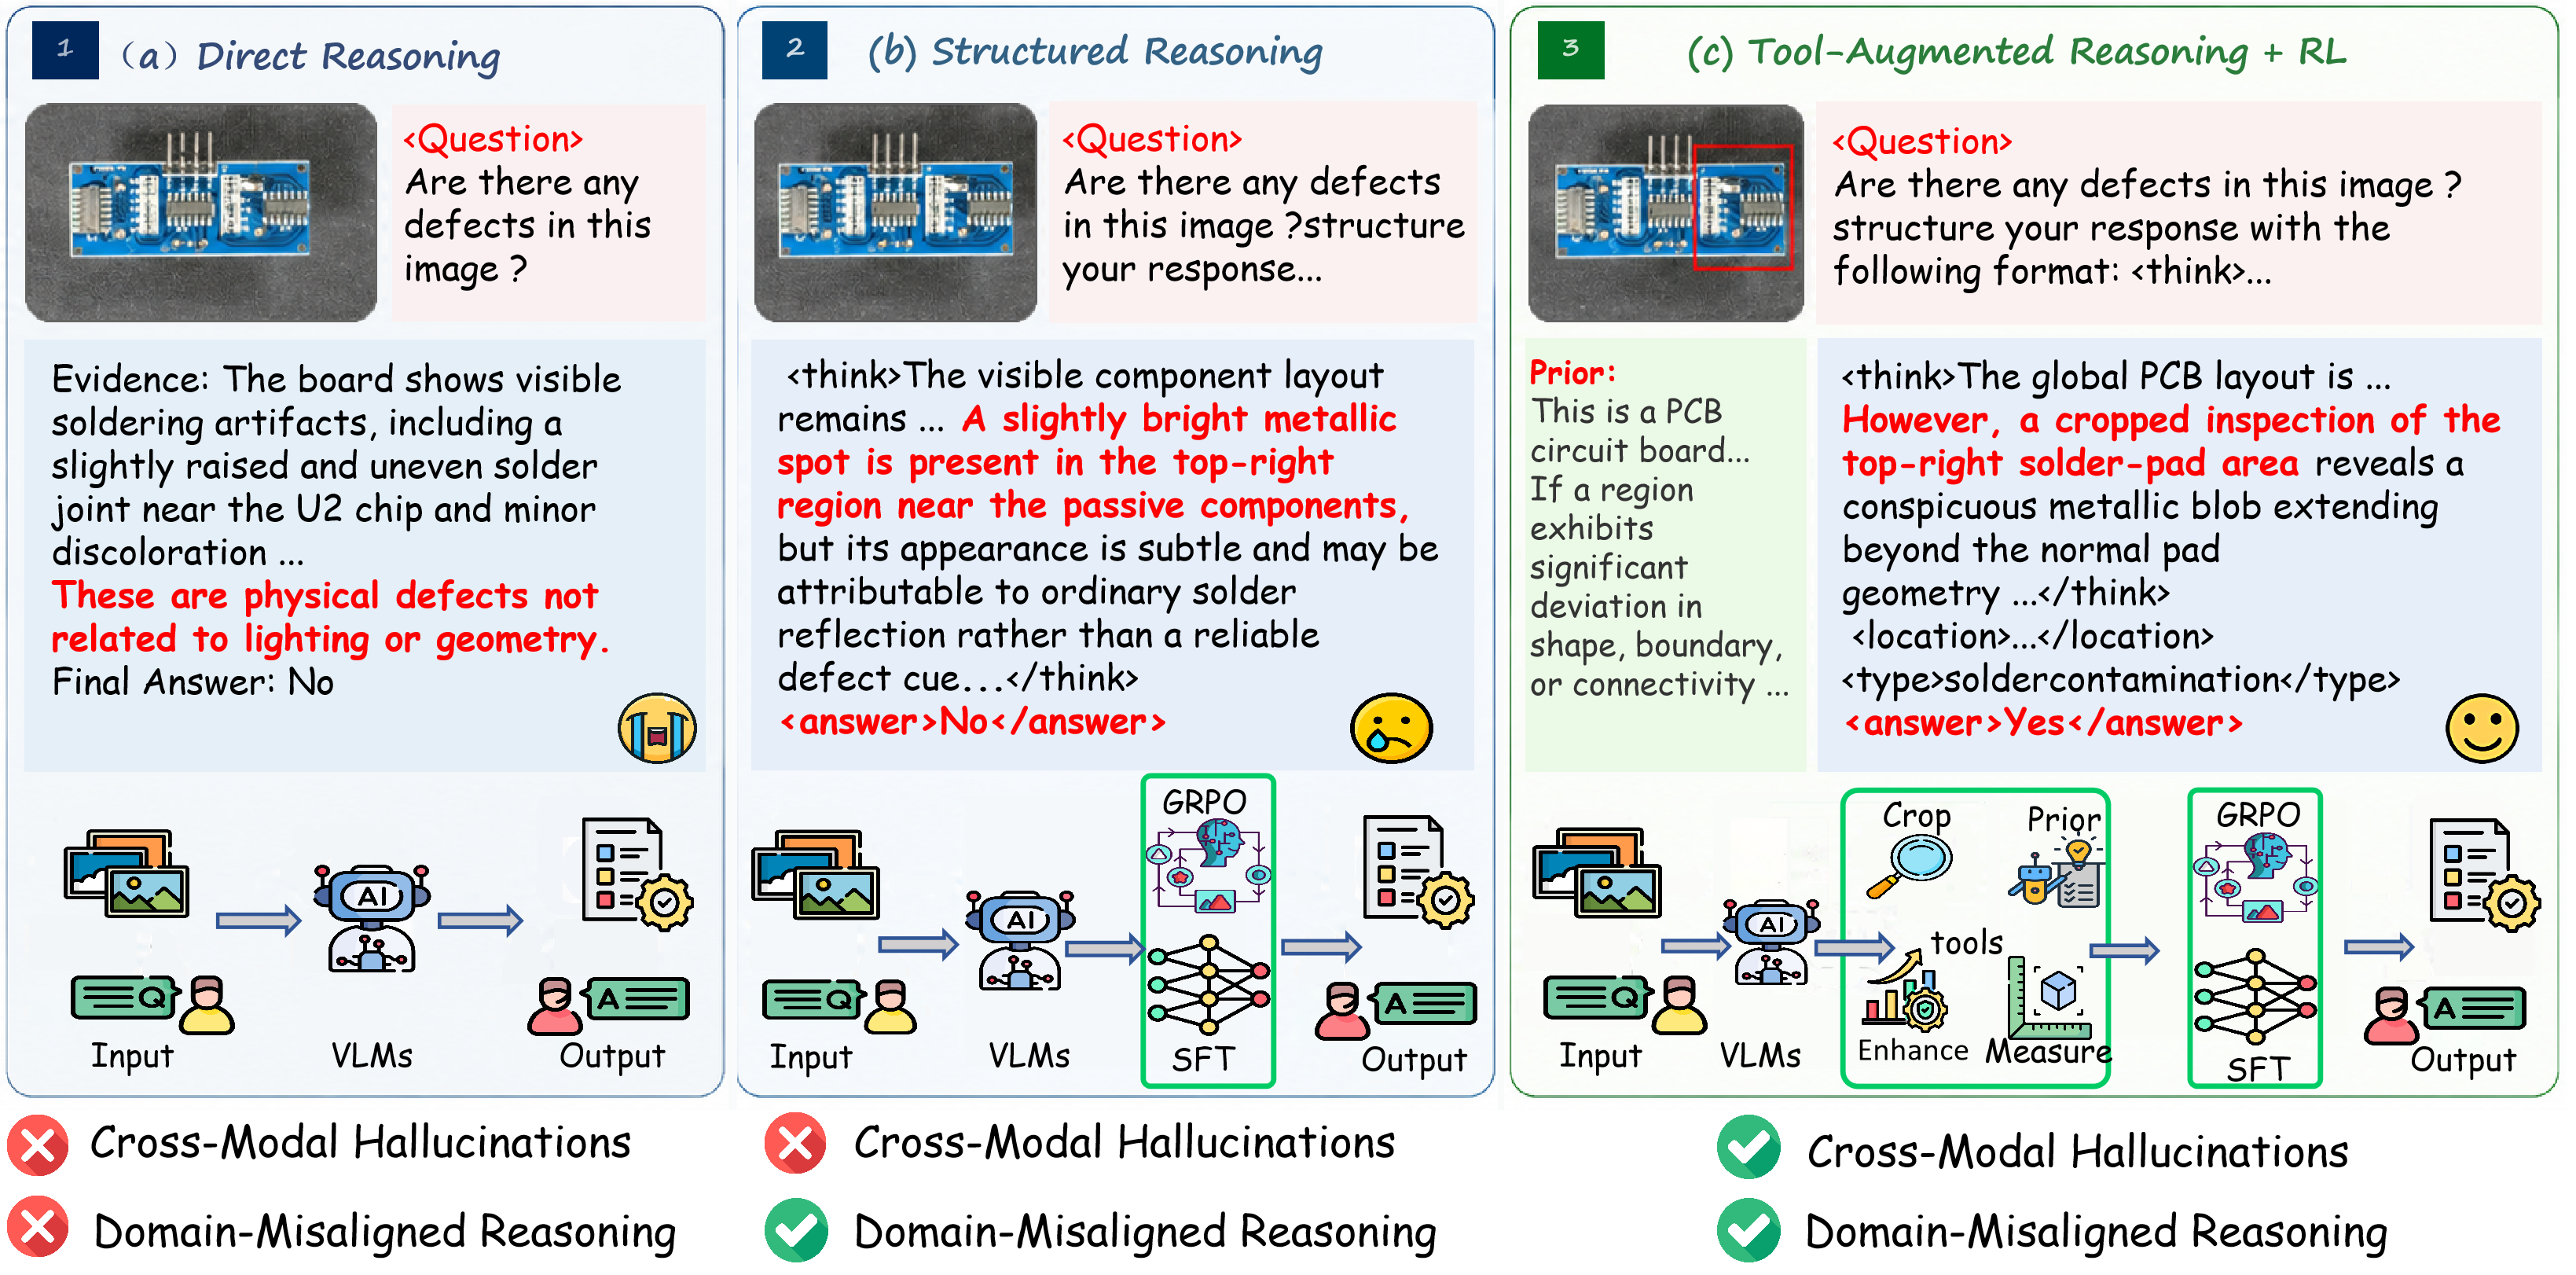
\includegraphics[width=\linewidth]{fig/intro16.png}
  \caption{\textbf{Comparison of anomaly detection paradigms using MLLMs.} (a) Standard MLLMs suffer from unaligned reasoning and structural hallucinations, often misinterpreting legitimate variations. (b) Ordinary Chain-of-Thought (CoT) reasoning is insufficient; without domain knowledge and localized perception, the model misjudges subtle defects as normal reflections due to perceptual dilution. (c) Our proposed framework constructs an active inspection paradigm through comprehensive tool orchestration. By synergizing high-resolution region cropping, low-level texture enhancement, quantitative geometric measurement, and expert semantic priors, the agent effectively overcomes both visual ambiguities and physical scale-blindness. This strategic alignment ensures rigorous diagnostic trajectories, accurately disentangling complex geometries to detect subtle anomalies.}
  \vspace{-0.2in}
  \label{fig:1}
\end{figure}

Open-vocabulary industrial anomaly detection (IAD) aims to identify unpredictable defect classes and unseen object categories not present during training, extending beyond the closed-set constraints of traditional visual inspection systems~\citep{mvtec, visa}. This capability is crucial for real-world manufacturing, where novel products and unpredictable defect morphologies frequently emerge.~\citep{tao2022deep, jeong2023winclip}. Mainstream non-LLM approaches, such as reconstruction-based networks (e.g., Autoencoders~\citep{zavrtanik2021draem, bergmann2018improving}, Diffusion models~\citep{wyatt2022anoddpm, mu2023diffusionad}) and feature-embedding frameworks (e.g., Memory banks~\citep{roth2022patchcore, defard2021padim}, Normalizing flows~\citep{yu2021fastflow, rudolph2022csflow}), are fundamentally bottlenecked by closed-set assumptions. They demand extensive category-specific normal data and critically lack the capacity to generalize to unseen products in open-world manufacturing scenarios~\citep{gu2024anomalygpt}.

Recently, the advent of Multimodal Large Language Models (MLLMs) has ignited a paradigm shift toward open-vocabulary visual reasoning~\citep{gpt4v}. By aligning visual tokens with rich textual semantics, MLLMs offer a transformative opportunity to overcome the data-dependency and closed-set limitations of traditional IAD systems, enabling unprecedented zero-shot detection capabilities.

However, bridging the cognitive gap between MLLMs and high-precision industrial applications reveals three intrinsic limitations: \ding{182} \textbf{Domain-Misaligned Reasoning:} As shown in Fig.~\ref{fig:1}(a), standard MLLMs are primarily optimized for open-ended, general-purpose conversations~\citep{liu2024visual}. Their inherent reasoning trajectories fail to conform to the strict, formalized diagnostic protocols that are essential for accurate industrial anomaly detection. \ding{183} c \ding{184} \textbf{Open-Vocabulary Generalization:} While existing models can memorize predefined defect categories, they exhibit brittle adaptability in open-vocabulary inspections. When confronting novel anomalies or ambiguous linguistic instructions, their zero-shot reasoning heavily deteriorates due to an inherent lack of strategic exploration and structural coherence~\citep{deepseekr1}.

% Fig.~\ref{tool}

To address these critical bottlenecks, we propose \textbf{IndusAgent}, a unified framework that synergizes domain-specific reasoning with autonomous tool orchestration. As shown in Fig.~\ref{fig:1}(c), We bridge the diagnostic protocol gap through \textbf{Supervised Fine-tuning}, which aligns the model's reasoning trajectories with expert-level industrial standards. Building on this foundation, we introduce \textbf{Tool Augmentation} into the agent's cognitive loop. This equips the model with the active means to combat perceptual dilution and structural hallucinations by dynamically scrutinizing high-resolution patches and querying expert normalcy priors. 

Furthermore, adapting to the boundless variations inherent in open-vocabulary IAD requires dynamic, self-improving exploration beyond static SFT. To this end, we introduce \textbf{Agentic Reinforcement Learning (RL)} to optimize the agent's decision-making trajectories across unseen domains. However, empowering the agent with autonomous exploration inevitably risks \emph{tool abuse}—a prevalent issue where indiscriminate API invocations introduce redundant noise and dilute the reasoning focus. To overcome this dilemma without stifling necessary exploration, our RL framework features a novel \textbf{Accuracy-Gated} reward mechanism. By strictly gating a positive tool utility bonus with the final diagnostic correctness, this sophisticated formulation trains the agent to treat tool-calling as a high-stakes diagnostic instrument. It ensures that unbounded visual exploration is organically aligned with genuine diagnostic information gain~\citep{schick2024toolformer, zeng2024agenttuning}.

In summary, our main contributions are summarized as follows:
\begin{itemize}[leftmargin=*,nosep]
    \item \textbf{Active Inspector Paradigm.} We introduce a unified paradigm that integrates autonomous, multi-round tool orchestration with MLLMs for industrial anomaly detection, effectively transcending the resolution and semantic limitations inherent in passive visual perception.
    \item \textbf{Tool-Integrated Industrial Reasoning Corpus.} 
    We construct \emph{Indus-CoT}, a structured reasoning dataset that encodes industrial inspection trajectories with global observations, localized evidence, normalcy priors, and final defect judgments. 
    By explicitly linking visual cues, tool feedback, and diagnostic decisions, Indus-CoT provides effective supervision for domain-aligned, tool-augmented anomaly reasoning.
    \item \textbf{Accuracy-Gated Reward Mechanism.} We formulate a cascading Agentic RL objective that utilizes a multiplicative gate to seamlessly integrate tool utility with diagnostic task efficacy. By rewarding tool orchestration \emph{only} when it culminates in correct predictions, this design successfully eradicates stochastic tool abuse and fosters a highly judicious, accuracy-driven reasoning policy.
    \item \textbf{State-of-the-Art Performance.} IndusAgent achieves state-of-the-art results across five challenging benchmarks (MVTec-AD, VisA, DTD, MPDD, and SDD), especially outperforming SOTA method by $9.3\%$ on MVTec, validating our effectiveness. 
    % Our framework redefines the performance ceiling for complex industrial inspection by empowering models with unbounded yet highly effective evidence-gathering capabilities.
\end{itemize}


\section{Methodology}

\begin{figure} [!t]
  \centering
  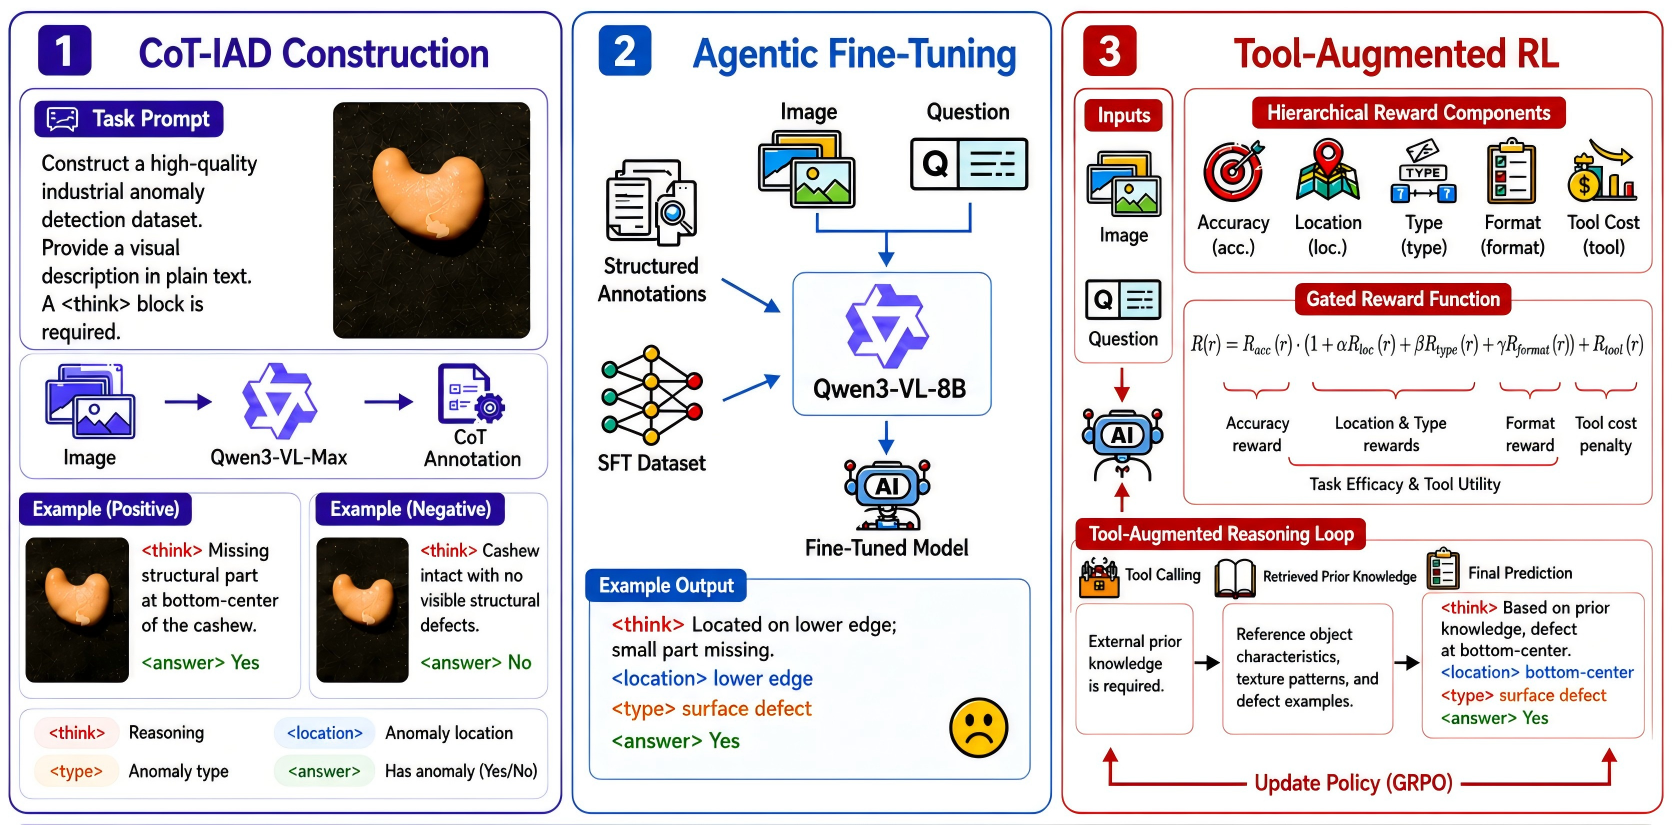
\includegraphics[width=\textwidth]{fig/overview12.png }
  \caption{\textbf{The overall architecture of IndusAgent.} Our training pipeline consists of three sequential stages: \textbf{(1) Indus-CoT Construction}, where a frontier model (Qwen3-VL-Max) synthesizes structured reasoning trajectories to form high-quality positive and negative examples; \textbf{(2) Agentic Fine-Tuning}, which aligns a lightweight base model (Qwen3-VL-8B) with domain-specific diagnostic protocols; and \textbf{(3) Tool-Augmented RL}. In the final stage, the agent's tool-augmented reasoning loop is optimized via GRPO. The policy is guided by a specific gated reward function $R(r)$.}
  \label{fig:overview1}
\end{figure}

\textbf{Overview.}
We propose IndusAgent, a post-training framework that synergizes visual anomaly perception with tool-augmented reinforcement learning, as illustrated in Fig.~\ref{fig:overview1}. The framework consists of three tightly coupled stages. First, we construct \textbf{Indus-CoT}, a tool-integrated reasoning dataset that synthesizes image-query trajectories with predefined prompts to bridge visual perception and tool execution~\citep{wei2022chain, liu2024visual}. Second, we perform \textbf{Supervised Fine-Tuning} to align the VLM with structured industrial diagnostic trajectories and tool-use syntax. Third, we apply \textbf{Tool-Augmented Reinforcement Learning} with a hierarchical reward that jointly balances tool-usage correctness, anomaly interpretation, and structural reasoning coherence~\citep{ouyang2022training}.

\subsection{Systematic Definition and Agentic Toolkit}
\label{sec:Formulation}

\textbf{Problem Formulation.} 
We formulate industrial anomaly detection (IAD) as a tool-augmented visual reasoning process~\citep{gupta2023visual}. 
Given only a query image $I \in \mathbb{R}^{H \times W \times 3}$ and a task instruction $Q$, the model is required to generate a structured diagnostic output $O$, including the reasoning trajectory, anomaly localization, fine-grained defect category, and final binary judgment. 
All models, including commercial APIs and open-source baselines, receive the same query image and textual instruction, and are required to infer the normal structure and anomaly status from their internal visual-language knowledge and the provided input alone.
Instead of directly mapping the input image to a prediction, we instantiate the VLM as an agentic policy $\pi_\theta$ based on Qwen3-VL-8B~\citep{Qwen3-VL}.  
The policy interacts with a customized tool space 
$\mathcal{T}=\{T_{\text{crop}},T_{\text{prior}},T_{\text{enhance}},T_{\text{measure}}\}$ 
to actively acquire complementary evidence for diagnosis.

\textbf{Unified Agentic Inference.} 
IndusAgent performs diagnosis through a multi-step autoregressive reasoning process. 
After perceiving the global image, the policy identifies uncertain regions or ambiguous structures and generates tool calls $C \subseteq \mathcal{T}$ when additional evidence is needed. 
The corresponding tool observations are then fused with the original image and instruction to produce the final structured output:
\begin{equation}
O \sim \pi_\theta(\cdot \mid I \oplus F, Q \oplus E; \mathcal{T}),
\end{equation}
where $\oplus$ denotes multimodal fusion. 
Here, $F$ represents visual feedback, including high-resolution local patches from $T_{\text{crop}}$ and enhanced texture maps from $T_{\text{enhance}}$, while $E$ denotes semantic or quantitative feedback, including normalcy priors from $T_{\text{prior}}$ and geometric measurements from $T_{\text{measure}}$. 
This formulation enables the agent to combine global context, localized evidence, and external diagnostic cues before making the final decision.

\textbf{Agentic Toolkit.}
We instantiate four tools to address typical IAD failure modes. $T_{\text{crop}}$ extracts high-resolution patches from suspicious regions to recover fine-grained defects diluted by global encoding. $T_{\text{prior}}$ retrieves normalcy priors describing defect-free geometry, texture, and structural patterns, providing a comparison anchor for distinguishing true defects from acceptable variations. $T_{\text{enhance}}$ applies lightweight image-processing operations, such as contrast enhancement and edge extraction, to highlight low-contrast texture changes. $T_{\text{measure}}$ computes geometric relations, such as distances, angles, and relative positions, to verify misalignment, deformation, missing parts, and abnormal spacing.

\subsection{Indus-CoT Dataset}
\label{sec:Training}

Existing VLMs face two major limitations in industrial anomaly detection: they passively observe the input image without actively seeking external evidence, and they may hallucinate defect explanations when subtle visual cues cannot be cross-verified with domain knowledge~\citep{driess2023palm, sun2024aligning}. 
To address these issues, we construct \textbf{Indus-CoT}, a tool-integrated reasoning dataset that combines multimodal CoT trajectories with explicit tool-execution traces~\citep{zhang2023multimodal, chen2023fireact}. 
This dataset provides supervision for multi-round diagnostic reasoning, where the model learns not only to judge anomalies but also to acquire and use external evidence when necessary.

\textbf{Data Collection \& Automated Curation.}
We sample images from Real-IAD~\citep{wang2024realiad} and construct about 3,000 reasoning trajectories, with roughly balanced normal and anomalous samples~\citep{wang2023selfinstruct}. 
To prevent category leakage, we remove all Real-IAD categories overlapping with the evaluation benchmarks, including DTD, MPDD, MVTec-AD, SDD, and VisA, using both exact matching and semantic normalization for naming variants such as \texttt{pcb} versus \texttt{pcb1}/\texttt{pcb2}/\texttt{pcb3}/\texttt{pcb4} and \texttt{transistor1} versus \texttt{transistor}. 
After filtering overlapping categories such as \texttt{toothbrush}, \texttt{zipper}, \texttt{pcb}, and \texttt{transistor1}, the resulting training set is category-disjoint from all test benchmarks.

For each query image, no paired normal reference image is provided to the teacher model. 
The teacher receives only the query image and task instruction, infers the expected defect-free appearance from its internal visual-language knowledge and general industrial priors, and generates a structured \texttt{Indus-CoT} trajectory covering global perception, tool routing, tool observations, and final diagnostic verification. 
This reference-free construction matches our inference setting, where both IndusAgent and all baselines diagnose anomalies from the query image alone. 
To improve data quality, we further apply self-correction and LLM-as-a-judge validation to repair invalid outputs, score candidate trajectories, and retain the highest-quality valid trajectory, thereby reducing label inconsistency and formatting errors in the SFT data.

\textbf{Tool-Integrated Generating Pipeline.}
Indus-CoT trajectory follows a three-phase reasoning process:
\begin{itemize}[leftmargin=*,nosep]
    \item \textbf{Phase 1: Global Perception and Tool Routing.} 
    The model first analyzes the global query image to identify suspicious regions, ambiguous structures, or uncertain visual patterns. 
    Instead of directly producing a final judgment, it generates routing commands to invoke suitable tools.

    \item \textbf{Phase 2: Tool Execution and Contextual Observation.} 
    The selected tools return complementary observations. 
    $T_{\text{prior}}$ provides textual normalcy priors, $T_{\text{measure}}$ computes distances or angles from specified coordinates, and $T_{\text{enhance}}$ applies deterministic filters such as CLAHE to highlight high-frequency textures. 
    For $T_{\text{crop}}$, we avoid using ground-truth boxes during execution and instead adopt an unsupervised foreground extraction procedure, combining background estimation, image differencing, Otsu thresholding, morphological operations, and a center-crop fallback.

    \item \textbf{Phase 3: Final Diagnostic Verification.} 
    The model integrates the original image with tool observations, including local crops, enhanced texture maps, normalcy priors, and geometric measurements. 
    It then cross-verifies the collected evidence and outputs the final anomaly judgment, location, and defect category.
\end{itemize}

\subsection{Supervised Fine-Tuning}
\label{sec:SFT}

Directly optimizing Vision-Language Models with reinforcement learning for complex visual tasks is often unstable. Inspired by R1-Zero~\citep{guo2025deepseek}, our preliminary trials show that, without structural constraints, the policy can suffer from \emph{reward hacking} and \emph{format collapse}, bypassing intermediate visual inspection and exploiting terminal rewards through blind binary guesses. To stabilize training, we introduce a \textbf{Supervised Fine-Tuning (SFT)} stage to cold-start Qwen3-VL-Instruct (8B) with structured industrial diagnostic trajectories before reinforcement learning.

Formally, we formulate SFT as conditional autoregressive generation over our curated reasoning dataset. Each training instance is denoted as $\mathcal{T} = (\mathcal{X}, \mathcal{I}, \mathcal{S}, \mathcal{Y})$, where $\mathcal{X}$ denotes the visual input, including the global query image and multi-round tool observations; $\mathcal{I}$ is the task instruction; $\mathcal{S}=\{s_1,\dots,s_T\}$ represents the reasoning steps constrained within the \texttt{<think>\dots</think>} trajectory; and $\mathcal{Y}$ denotes the final target output.

To guarantee that the model actively internalizes the reasoning logic rather than passively memorizing the input context, we implement a selective masking strategy during training. The objective minimizes the negative log-likelihood exclusively over the generated tokens of the reasoning process:
\begin{equation}
\mathcal{L}_{\text{SFT}} = -\mathbb{E}_{\mathcal{T} \sim \mathcal{D}} \left[ \sum_{t=1}^{T} \log p_{\theta}(s_t \mid \mathcal{X}, \mathcal{I}, s_{<t}) \right],
\end{equation}
where $p_{\theta}(\cdot)$ dictates the conditional probability distribution of the parameterized policy network. By explicitly supervising the cognitive trajectory, this phase successfully anchors the model's structural consistency, equipping it with a robust and well-calibrated policy initialization for the subsequent reinforcement learning phase.

\subsection{Agentic Reinforcement Learning}
\label{sec:RL}

\textbf{Group Relative Policy Optimization (GRPO).}
To optimize the agent's decision-making process without the prohibitive memory costs associated with traditional actor-critic architectures~\citep{schulman2017proximal}, we utilize Group Relative Policy Optimization (GRPO)~\citep{shao2024deepseekmath}. Instead of relying on a separate value network, GRPO evaluates policy updates through a groupwise relative comparison mechanism.
Specifically, for a given query image $ q $ and its corresponding ground truth $ a $ sampled from the dataset $ D $, the system samples a batch of $ G $ distinct reasoning trajectories $ \{o_1, o_2, \dots, o_G\} $ using the reference policy $ \pi_{\theta_{\text{old}}} $. The current policy $ \pi_\theta $ is subsequently updated by maximizing the following:  

% ##########################################################
% \begin{equation}
% \begin{split}
% \mathcal{L}_{GRPO}(\theta) = &-\mathbb{E}_{q \sim P(Q), \{o_i\}_{i=1}^{G} \sim \pi_{\theta_{old}}(O|q)} \Bigg[ \frac{1}{G} \sum_{i=1}^G
% & \Bigg ( \min\bigg( \frac{\pi_\theta(o_i|q)}{\pi_{\theta_{old}}(o_i|q)} A_i,
% \text{clip}\Big(\frac{\pi_\theta(o_i|q)}{\pi_{\theta_{old}}(o_i|q)}, 1-\epsilon, 1+\epsilon\Big) A_i \bigg)
% & - \beta \mathbb{D}_{KL}(\pi_\theta || \pi_{ref}) \Bigg) \Bigg],
% \end{split}
% \end{equation}

\begin{equation}
\begin{aligned}
    &\mathcal{L}_{GRPO}(\theta) = -\mathbb{E}_{q \sim P(Q), \{o_i\}_{i=1}^{G} \sim \pi_{\theta_{old}}(O|q)} \Bigg[ \frac{1}{G} \sum_{i=1}^G \\
    &\quad \Bigg( \min\left( \frac{\pi_\theta(o_i|q)}{\pi_{\theta_{old}}(o_i|q)} A_i, \text{clip}\left(\frac{\pi_\theta(o_i|q)}{\pi_{\theta_{old}}(o_i|q)}, 1-\epsilon, 1+\epsilon\right) A_i \right) - \beta \mathbb{D}_{KL}(\pi_\theta \| \pi_{ref}) \Bigg) \Bigg],
\end{aligned}
\end{equation}
% ##########################################################


\begin{equation}
\mathbb{D}_{KL}(\pi_\theta||\pi_{ref}) = \frac{\pi_{ref}(o_i|q)}{\pi_\theta(o_i|q)} - \log \frac{\pi_{ref}(o_i|q)}{\pi_\theta(o_i|q)} - 1, 
\end{equation}
where the coefficient $ \beta $ regulates the KL divergence penalty to ensure training stability and prevent the policy from deviating excessively from the reference model. The advantage estimator $ A_{i} $ is dynamically derived by normalizing the rewards within the sampled trajectory group:  
\begin{equation}
A_{i} = \frac{r_i - \text{mean}(\{r_1, r_2, \dots, r_G\})}{\text{std}(\{r_1, r_2, \dots, r_G\})}.
\end{equation}
Here, $ r_i $ represents the comprehensive scalar reward assigned to each trajectory $ o_i $, computed by a rigorous, rule-based verification mechanism to prevent reward hacking.

\textbf{Reward Formulation.}
A carefully designed reward is essential for encouraging effective tool use while avoiding behavioral degradation. 
We propose an \emph{Accuracy-Gated} reward that couples tool usage with final diagnostic correctness, so that auxiliary rewards are activated only when the basic anomaly judgment is correct.For a trajectory $\tau$, the overall reward is defined as:
\begin{equation}
R(\tau) =
R_{\text{acc}}(\tau)
\cdot
\Big(
1 + \alpha R_{\text{loc}}(\tau)
+ \beta R_{\text{type}}(\tau)
+ \gamma R_{\text{tool}}(\tau)
\Big)
+
R_{\text{format}}(\tau),
\end{equation}
where $R_{\text{acc}}$ denotes binary anomaly classification correctness, $R_{\text{loc}}$ measures localization quality, $R_{\text{type}}$ evaluates fine-grained anomaly categorization, $R_{\text{tool}}$ encourages useful tool invocation, and $R_{\text{format}}$ enforces output-format compliance. 
The weights $\alpha$, $\beta$, and $\gamma$ balance the relative contributions of localization, semantic categorization, and tool usage.

\ding{182} \textbf{Classification Accuracy ($R_{\text{acc}}$):} $R_{\text{acc}} \in \{0,1\}$ evaluates whether the final binary anomaly judgment is correct and serves as a multiplicative gate, ensuring that localization, type prediction, and tool-usage rewards are credited only when the final diagnosis is correct. \ding{183} \textbf{Spatial Localization ($R_{\text{loc}}$):} $R_{\text{loc}}$ measures the overlap between the predicted anomaly region and the ground-truth region using IoU. \ding{184} \textbf{Semantic Categorization ($R_{\text{type}}$):} $R_{\text{type}}$ evaluates the correctness of the predicted anomaly type based on its semantic distance to the ground-truth category. \ding{185} \textbf{Tool Utility ($R_{\text{tool}}$):} To promote useful rather than excessive tool use, we define $R_{\text{tool}}=\lambda \cdot \mathbb{I}[\Delta_{\text{conf}}>0]-\eta|C|$, where $C$ is the set of invoked tools, $\Delta_{\text{conf}}$ denotes the confidence improvement after incorporating tool feedback, $\mathbb{I}[\cdot]$ is the indicator function, $\lambda$,$\eta$ are hyperparameters, empirically set to 0.3 and 0.1, respectively. This term rewards beneficial evidence acquisition while penalizing redundant tool calls. \ding{186} \textbf{Process Compliance ($R_{\text{format}}$):} $R_{\text{format}}$ penalizes invalid output structures, such as missing or malformed \texttt{<answer>} tags, to prevent format collapse during RL training.


% \begin{itemize}[leftmargin=*,nosep]

%     \item \textbf{Task Gain \& Multiplicative Gating:} This term captures the core diagnostic performance. $R_{\text{acc}} \in \{0, 1\}$ evaluates the fundamental binary anomaly classification. Crucially, it acts as a \emph{multiplicative gate} for all advanced metrics. If the foundational binary judgment is incorrect ($R_{\text{acc}} = 0$), the agent receives zero credit for spatial localization ($R_{\text{loc}}$), fine-grained categorization ($R_{\text{type}}$), or tool usage ($R_{\text{tool}}$). This effectively eradicates rewards for hallucinated defects and blind guessing.
%     \item \textbf{Process Compliance:} $R_{\text{format}}$ provides a baseline reward strictly penalizing deviations from the required structural syntax, applied independently of the diagnostic outcome to prevent format collapse.
%     \item \textbf{Tool Utility ($R_{\text{tool}}$):} Instead of explicitly penalizing the cost of tool execution, we introduce a positive utility bonus for invoking external tools. Because this bonus resides strictly within the $R_{\text{acc}}$ gate, the agent is rewarded for tool orchestration \emph{only if} the trajectory culminates in a correct final prediction.
% \end{itemize}

\textbf{Effect on Tool-Use Behavior.}
The accuracy-gated formulation encourages the agent to associate tool use with final diagnostic correctness rather than tool invocation itself. 
Since $R_{\text{tool}}$ contributes to the reward only when the binary anomaly judgment is correct, redundant or uninformative tool calls do not provide effective task-level gains and are further penalized by the cost term $-\eta |C|$. 
As a result, the policy is biased toward invoking tools only when additional local, textual, or geometric evidence is likely to improve the final diagnosis.


\section{Experiment}


\subsection{Experimental Setup}
\label{sec:experiments_setup}

\textbf{Datasets and Benchmarks.}
We evaluate \textbf{IndusAgent} on five industrial anomaly detection benchmarks: MVTec-AD~\citep{mvtec}, VisA~\citep{visa}, MPDD~\citep{mpdd}, DTD~\citep{dtd}, and SDD~\citep{sdd}. 
These datasets comprehensively cover two representative scenarios: (1) \textcolor{teal}{\emph{industrial objects}}, which are characterized by complex structures, poses, and geometries; (2) \textcolor{orange}{\emph{surface textures}}, where defects are often subtle and embedded within repetitive or noisy patterns. 
To ensure a fair comparison, all baselines are evaluated under identical prompt and answer parsing protocols.

%%%%%%%%%%%%%%%%%%%%%%%%%%%%%%%%%%%% revise 
% 个人感觉分数据集分部分的时候可以用标号，增加审稿人的视觉区分度，至于是否需要加颜色更清晰表示随意，因为后面部分还有一些空余，适当补充几行Implementation Details. comprehensively修饰一下cover，加强对实验覆盖面的广泛性的强调。which involve可以替换which are characterized by（以...为特征），描述数据集特性时更具体一些，当然我对数据集的性质不太了解，可换可不换。under the same可替换under identical，在描述类似这样语境的词汇的时候尽量找一些专业的学术表达，避免口语化的说法。

% \textbf{Datasets and Benchmarks.}
% We evaluate \textbf{IndusAgent} on five industrial anomaly detection benchmarks: MVTec-AD~\citep{mvtec}, VisA~\citep{visa}, MPDD~\citep{mpdd}, DTD~\citep{dtd}, and SDD~\citep{sdd}. 
% These datasets comprehensively cover two representative scenarios: (1) \textcolor{teal}{\emph{industrial objects}}, which are characterized by complex structures, poses, and geometries; (2) \textcolor{orange}{\emph{surface textures}}, where defects are often subtle and embedded within repetitive or noisy patterns. 
% To ensure a fair comparison, all baselines are evaluated under identical prompt and answer parsing protocols.

% \textbf{Implementation Details. }
% ... 
%%%%%%%%%%%%%%%%%%%%%%%%%%%%%%%%%%%% revise 





\begin{table*}[t]
\centering
\caption{Performance comparison of different models on industrial workpieces and surface texture benchmarks. The \colorbox{best2}{best} and \colorbox{best}{second best} results are highlighted.}
\label{model_comparison}
\resizebox{\textwidth}{!}{
\begin{tabular}{l|lc|ccc|ccc|c}
\toprule
\multicolumn{1}{c|}{\multirow{2}{*}{Type}} &
\multicolumn{1}{c}{\multirow{2}{*}{Model}} &
\multicolumn{1}{c|}{\multirow{2}{*}{Param.}} &
\multicolumn{3}{c|}{\textbf{Industrial Workpieces}} &
\multicolumn{2}{c|}{\textbf{Surface Texture}} &
\multicolumn{1}{c}{\multirow{2}{*}{Avg.}} \\
\cmidrule(lr){4-6} \cmidrule(lr){7-8}
& & & MVTec & MPDD & VisA &  DTD & SDD & \\
\midrule

\multirow{6}{*}{Commercial}
& GPT-4o-mini~\cite{openai2024gpt4o} & / & 71.3 & 67.9 & 65.1  & 79.5 & 66.6 & 70.1 \\
& GPT-4o ~\cite{openai2024gpt4o}& / & 69.6 & 60.3 & 63.5  & 69.9 & 65.7 & 65.8 \\
& GPT-4.1-nano~\cite{openai2025gpt41} & / & 74.7 & 61.7 & 60.5  & 78.3 & 50.0 & 65.0 \\
& GPT-4.1-mini~\cite{openai2025gpt41} & / & 74.0 & 69.8 & 63.4  & 82.1 & 72.1 & 72.3 \\
& GPT-4.1~\cite{openai2025gpt41} & / & 81.9 & 66.7 & 69.1  & 90.1 & 79.9 & 77.5 \\
& Claude-Sonnet-4~\cite{anthropic2025claude4} & / & 67.6 & 65.9 & 63.5  & 88.4 & 81.7 & 73.4 \\

\midrule
\multirow{12}{*}{Open Source}
& LLaVA-OneVision-SI~\citep{li2024llavaonevision} & 0.5B & 50.0 & 50.0  & 50.0 & 54.3 & 50.0 & 50.8 \\
& Anomaly-OV~\citep{xu2025towards} & 0.5B & 50.0  & 50.0 & 50.0 & 53.8 & 50.0 & 50.8 \\
& Qwen2.5-VL-Instruct~\citep{Qwen2.5-VL} & 3B & 62.6 & 52.9 & 58.4  & 64.4 & 50.3 & 57.7 \\
& AnomalyR1\cite{chao2025anomalyr1} & 3B & 69.4 & 56.0 & 59.8  & 61.0 & 57.6 & 60.7 \\
& InternVL-2.5~\citep{chen2024internvl} & 4B & 56.6 & 59.1 & 53.7  & 81.3 & 64.1 & 62.9 \\
& Qwen2.5-VL-Instruct~\citep{Qwen2.5-VL} & 7B & 66.0 & 56.0 & 58.4  & 59.2 & 67.4 & 61.4 \\

& Qwen3-VL-Instruct ~\citep{Qwen3-VL}& 8B & 67.0 & 50.0 & 46.8  & 70.2 & 50.0 & 56.8 \\

& AnomalyGPT~\citep{gu2024anomalygpt} & 7B & 46.6 & 54.2 & 57.3  & 64.1 & 49.5 & 54.3 \\

& Anomaly-OV~\citep{xu2025towards} & 7B & 74.3 & \cellcolor{best}70.3 &\cellcolor{best} 74.3  & \cellcolor{best}90.7 & \cellcolor{best}88.7 & 79.6 \\
& LLaVA-1.5~\citep{liu2023llava15} & 13B & 61.4 & 61.4 & 67.2 & 75.9 & 50.0 & 63.1 \\
& LLaVA-1.6~\citep{liu2024llavanext} & 34B & 53.7 & 50.0 & 53.9  & 52.7 & 50.0 & 52.0 \\
& Qwen2.5-VL-Instruct~\cite{Qwen2.5-VL} & 72B & 77.4\cellcolor{best} & 64.7 & 68.2  & 81.9 & 69.0 & 72.2 \\
\midrule
\multirow{1}{*}{}
& IndusAgent (Ours) & 8B &\cellcolor{best2} 83.6 &\cellcolor{best2} 72.7 & \cellcolor{best2}76.8 & \cellcolor{best2}95.6 & \cellcolor{best2}88.9 & 83.4 \\
\bottomrule
\end{tabular}
}
\end{table*}


\subsection{Main Results}


Table~\ref{model_comparison} and Figure~\ref{fig:radar} present a comprehensive zero-shot performance comparison across five industrial anomaly detection (IAD) benchmarks, encompassing both industrial objects and surface textures. Overall, our proposed \textbf{IndusAgent} (8B) establishes a new state-of-the-art (SOTA) with an average score of 83.4\%. As visually corroborated by its dominant envelope in the radar chart, it significantly and consistently outperforms both leading commercial systems and the largest open-source models. Notably, on structurally complex datasets such as VisA and MPDD, IndusAgent achieves impressive scores of 76.8\% and 72.7\%, respectively. This decisively surpasses the best-performing VLM baselines while strictly maintaining a highly efficient 8B parameter footprint. 

%%%%%%%%%%%%%%%%%%%%%%%%%%%%%%%%%%%% revise 
% 雷达图的“轨迹”用trajectory是规范的不？确认下是否可替换为envelope（包络线）或coverage。encompassing both structural workpieces and surface textures.这里原文用的是structural workpieces，但上一段刚刚定义了 industrial objects，是不是应该统一，另外如果统一的话感觉刚刚就介绍了dataset，重新叙述一下有点冗余，是不是可以考虑删掉这后面这半句。Notably这句有点太长了，一般写论文的时候很长的表达最好改成两三个短句表达，读起来会更舒服一些，考虑修改。

% Table~\ref{model_comparison} and Figure~\ref{fig:radar} present a comprehensive zero-shot performance comparison across five industrial anomaly detection (IAD) benchmarks, encompassing both industrial objects and surface textures. Overall, our proposed \textbf{IndusAgent} (8B) establishes a new state-of-the-art (SOTA) with an average score of 83.4\%. As visually corroborated by its dominant envelope in the radar chart, it significantly and consistently outperforms both leading commercial systems and the largest open-source models. Notably, on structurally complex datasets such as VisA and MPDD, IndusAgent achieves impressive scores of 76.8\% and 72.7\%, respectively. This decisively surpasses the best-performing VLM baselines while strictly maintaining a highly efficient 8B parameter footprint.
%%%%%%%%%%%%%%%%%%%%%%%%%%%%%%%%%%%% revise 

\begin{wrapfigure}{r}{0.35\textwidth} % 【核心修改】：将盒子宽度缩小至 35%
  % \vspace{-1.5em}
  \vspace{-1.5em} 
  \centering
  % 图片自动填满当前变小的盒子
  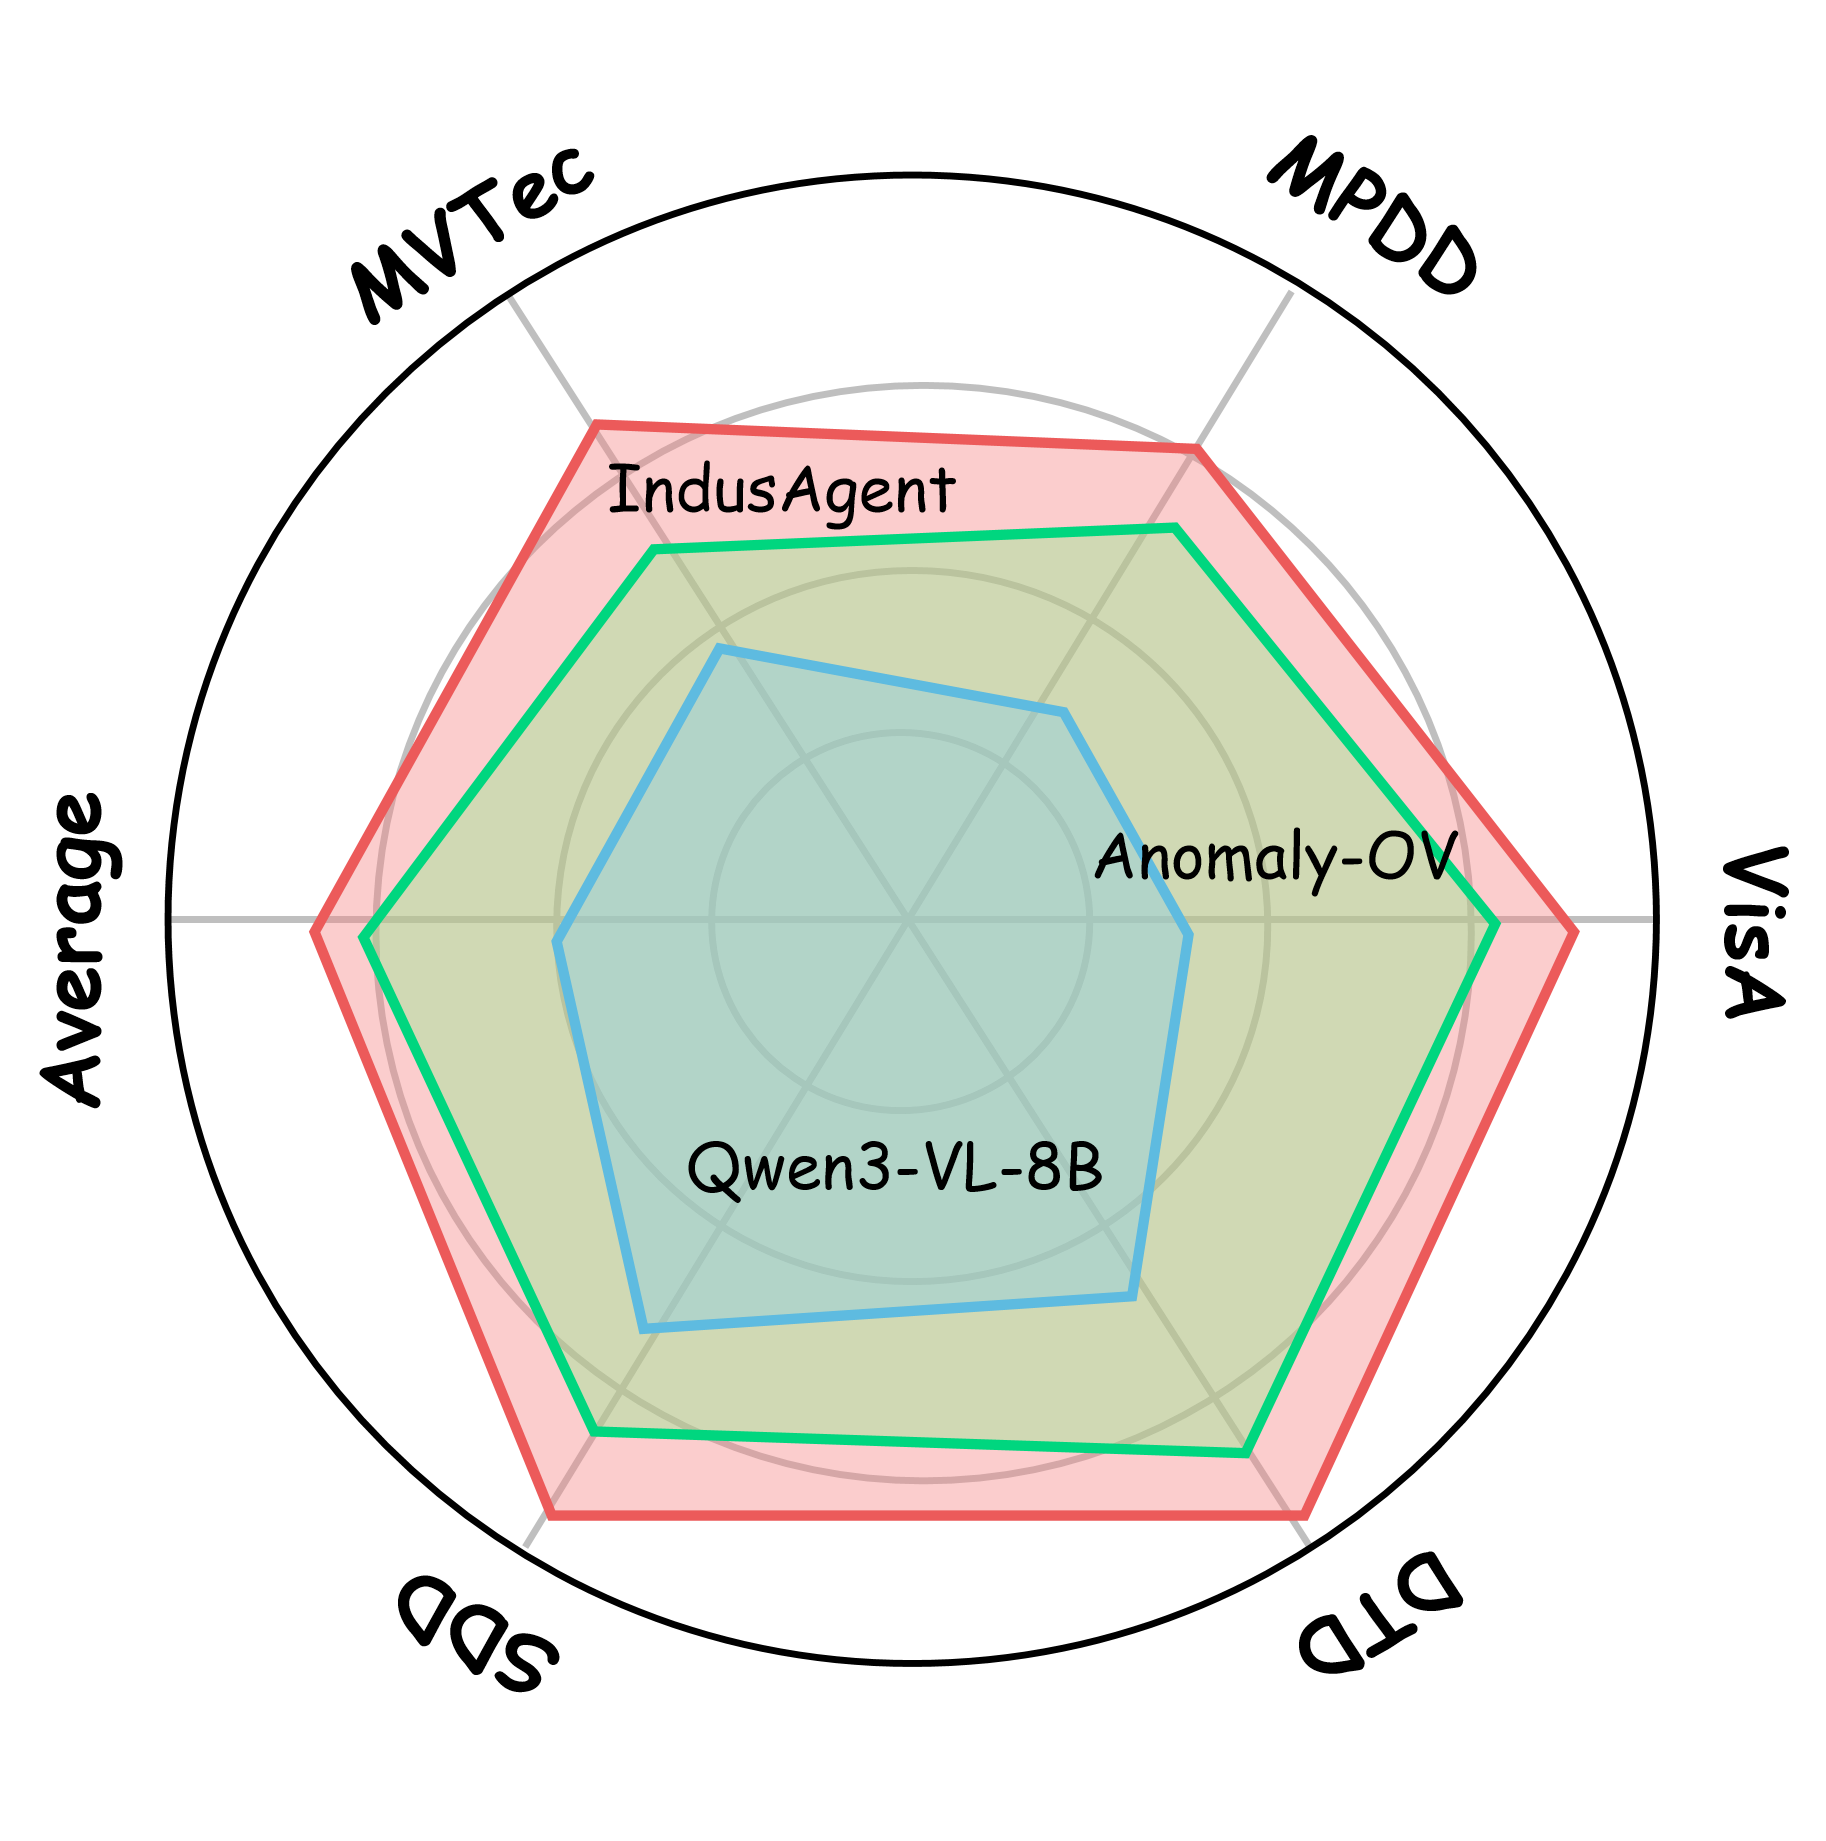
\includegraphics[width=\linewidth]{fig/show1.png} 
  \caption{\textbf{Zero-shot Comparison.}}
  \label{fig:radar}
  \vspace{-1.5em} 
\end{wrapfigure}

\subsection{Key Findings and Insights}

% Beyond the overall gains, our evaluation yields two key insights. 

\textbf{Finding 1: Domain-specific alignment is critical.}
MLLM reasoning alone remains unreliable for complex industrial samples. For example, Qwen3-VL-Instruct performs poorly on VisA, while Agentic SFT and RL substantially improve performance, indicating that robust IAD requires task-specific diagnostic alignment rather than open-ended reasoning alone.

\textbf{Finding 2: Active tooling complements passive perception.}
Subtle defects are often diluted by large normal regions, visual noise, or scale ambiguity. By selectively invoking cropping, enhancement, measurement, and normalcy-prior retrieval, IndusAgent isolates local evidence and verifies structural cues, showing that active tool use is an important complement to passive MLLM perception.



\begin{table*}[t]
\centering
\caption{Anomaly Recall Comparison. Our method fundamentally mitigates the false-negative bottleneck inherent in standard MLLMs. IndusAgent consistently outperforms both open-source models and commercial APIs, achieving massive recall surges and ensuring industrial-grade reliability.}
\label{tab:anomaly_recall}
% 移除 resizebox，改用精确的列间距控制和字号控制
\setlength{\tabcolsep}{8pt} 
\small % 设置为标准 9pt 字号
\begin{tabular}{l|ccccc|c}
\toprule
\multicolumn{1}{c|}{Model} & \multicolumn{1}{c}{DTD} & \multicolumn{1}{c}{MPDD} & \multicolumn{1}{c}{MVTec} & \multicolumn{1}{c}{SDD} & \multicolumn{1}{c|}{VisA} & \multicolumn{1}{c}{Avg.} \\
\midrule
Qwen3-VL-8B & 75.1\% & 62.3\% & 68.9\% & 64.2\% & 58.7\% & 65.8\% \\
Claude-Sonnet-4 & 80.2\% & 70.5\% & 75.3\% & 71.1\% & 65.4\% & 72.5\% \\
IAD-R1 &  \cellcolor{best}83.7\% &  \cellcolor{best}78.0\% &  \cellcolor{best}81.7\% &  \cellcolor{best}79.6\% &  \cellcolor{best}72.3\% &  \cellcolor{best}79.1\% \\
\midrule
IndusAgent (Ours) & \cellcolor{best2}94.1\% & \cellcolor{best2}95.4\% &\cellcolor{best2} 85.5\% & \cellcolor{best2}83.3\% & \cellcolor{best2}73.4\% & \cellcolor{best2}86.3\% \\
\bottomrule
\end{tabular}
\vspace{-1.0em}
\end{table*}


\textbf{Improvements in Anomaly Recall.} 
Anomaly recall is a critical metric in IAD, as missed defects (false negatives) typically incur higher costs than false alarms. As shown in Tab.~\ref{tab:anomaly_recall}, IAD-R1 model occasionally struggles with recall across various datasets. This suggests that conventional supervised fine-tuning may lead to conservative predictions, overlooking subtle defects in complex backgrounds. 

In contrast, our proposed GRPO framework addresses this limitation. By aligning the reasoning policy with final diagnostic outcomes, the agent is encouraged to actively verify potential anomalies rather than relying solely on initial passive observations. This approach yields consistent improvements in recall across all evaluated datasets. Notably, on datasets with severe background interference, the method shows substantial gains, achieving \textbf{+17.4\%} on MPDD and \textbf{+10.4\%} on DTD. These results demonstrate that the RL-driven orchestration effectively enhances the model's reliability for complex industrial inspection tasks.

\subsection{Ablation Studies}




To rigorously validate the contribution of each component, we conduct comprehensive ablation studies on three representative benchmarks. More ablation experiment results are shown in Appendix~\ref{appx:Experimentapp}.

\begin{wraptable}{r}{0.48\textwidth}
\vspace{-1.5em}
\centering
\caption{Ablation of main proposed modules.}
\label{table: Ablation_Macro}
\resizebox{\linewidth}{!}{
\footnotesize
\begin{tabular}{l|ccc}
\toprule
\multicolumn{1}{c|}{Method} & MVTec & VisA & DTD \\
\midrule
\emph{(a)} Qwen3-VL-8B & 67.0 & 46.8 & 70.2 \\
\emph{(b)} IndusAgent &\cellcolor{best2} 83.6 &\cellcolor{best2} 76.8 &\cellcolor{best2} 95.6 \\
\emph{(c)} w/o. \emph{RL} & 72.3 & 57.6 & 74.1 \\
\emph{(d)} w/o. \emph{SFT} & 69.5 & 55.5 & 72.8 \\
\emph{(e)} w/o. \emph{TOL} &  \cellcolor{best}78.1 &  \cellcolor{best}67.5 &  \cellcolor{best}87.9 \\
\bottomrule
\end{tabular}
}
\vspace{-1.0em}
\end{wraptable}

\textbf{Effectiveness of Core Framework Modules.} 
We first evaluate the macro-architecture by removing individual training stages. As shown in Table~\ref{table: Ablation_Macro}, omitting the Agentic Supervised Fine-Tuning phase (\emph{w/o. SFT}) leads to a catastrophic performance collapse (e.g., plunging from 76.8\% to 55.5\% on VisA). This confirms that domain-specific protocol alignment is an absolute prerequisite for industrial tasks. Similarly, removing Reinforcement Learning (\emph{w/o. RL}) results in a severe degradation, highlighting that SFT alone is insufficient for open-vocabulary generalization. Furthermore, ablating the Tool Augmentation library (\emph{w/o. TOL}) causes a noticeable drop across all datasets, empirically proving that active tool orchestration is vital for mitigating perceptual dilution and resolving complex structural hallucinations.



\begin{wraptable}{r}{0.48\textwidth}
\vspace{-1.5em}
\centering
\caption{Ablation of hierarchical gated rewards.}
\label{table: Ablation_Reward}
\resizebox{\linewidth}{!}{
\footnotesize
\begin{tabular}{l|ccc}
\toprule
\multicolumn{1}{c|}{RL Reward} & MVTec & VisA & DTD \\
\midrule
\emph{(f)} w/. \emph{Base} & 76.0 & 64.9 & 79.1 \\
\emph{(g)} w/o. \emph{Tool} & \cellcolor{best2}81.9 &  \cellcolor{best}71.5 &\cellcolor{best2} 92.8 \\
\emph{(h)} w/o. \emph{Loc} &  \cellcolor{best}79.5 & 68.8 & 89.6 \\
\emph{(i)} w/o. \emph{Type} & 78.5 &\cellcolor{best2} 72.8 & \cellcolor{best} 90.6 \\
\emph{(j)} w/o. \emph{Format} & 76.6 & 65.7 & 82.5 \\
\bottomrule
\end{tabular}
}
\vspace{-1.0em}
\end{wraptable}


\textbf{Deconstructing the Hierarchical Gated Reward.}
In Table~\ref{table: Ablation_Reward}, we dissect the Agentic RL phase to validate our hierarchical reward design. Compared to a standard RL baseline (\emph{w/. Base}), our full gated reward mechanism achieves consistently superior results. Notably, removing the format compliance reward (\emph{w/o. Format}) causes the most significant performance decay (e.g., dropping to 65.7\% on VisA), as structural reasoning breaks down without strict output parsing. Moreover, ablating the fine-grained diagnostic rewards (\emph{w/o. Loc} and \emph{w/o. Type}) impairs the model's ability to accurately ground anomalies in complex scenarios. Finally, removing the gated tool-utility term (\emph{w/o. Tool}) decreases accuracy, suggesting that explicitly coupling tool invocation with final diagnostic correctness helps the agent learn when external evidence is beneficial.

\begin{figure} [t]
  \centering
  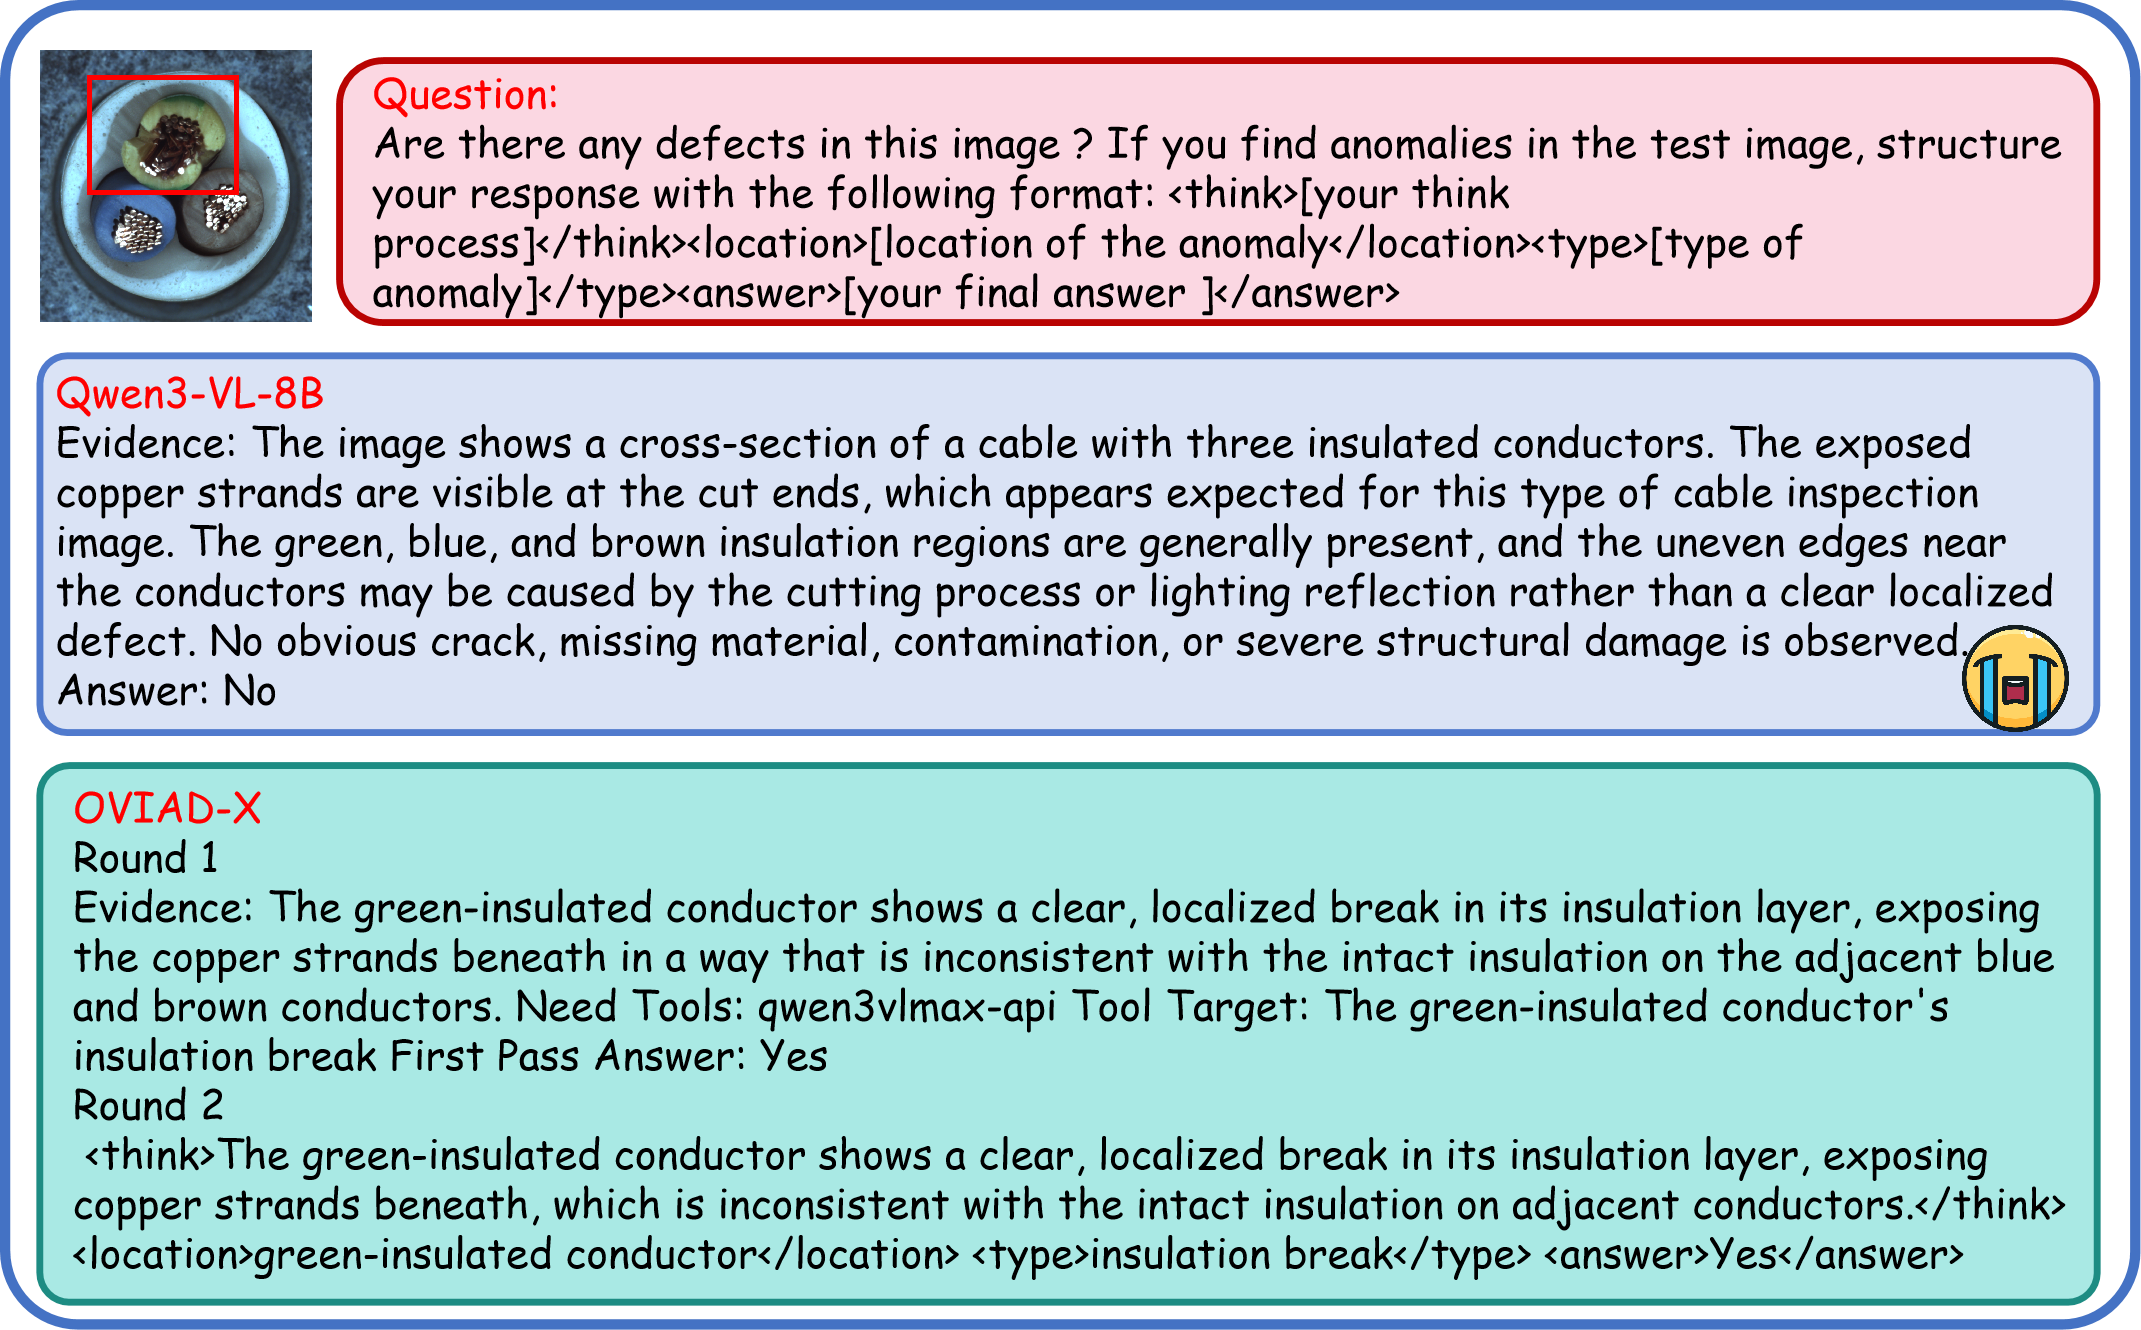
\includegraphics[width=\textwidth]{fig/case1.png }
   \caption{
    Case Study between Qwen3-VL-8B and our method.
    }
  \label{fig:case1}
  \vspace{-1.0em}
\end{figure}

\section{Related Work}

\textbf{Open-Vocabulary Industrial Anomaly Detection.}
OV-IAD methods span reconstruction-based, feature-embedding-based, and vision-language-based paradigms. Reconstruction approaches like DRAEM~\citep{zavrtanik2021draem} and autoencoder-based models~\citep{bergmann2018improving} learn normal appearance via inpainting or synthetic anomaly generation, while diffusion-based extensions like AnoDDPM~\citep{wyatt2022anoddpm} and DiffusionAD~\citep{mu2023diffusionad} improve reconstruction fidelity yet may reconstruct anomalies and miss subtle defects. Feature-embedding methods such as PaDiM~\citep{defard2021padim} and PatchCore~\citep{roth2022patchcore} achieve strong in-distribution performance through patch-level memory banks, while flow-based variants like FastFlow~\citep{yu2021fastflow} and CS-Flow~\citep{rudolph2022csflow} improve density estimation; yet both rely on closed-set assumptions limiting open-vocabulary applicability. Recent VLM-based approaches adapt cross-modal alignment for open-vocabulary inspection: WinCLIP~\citep{jeong2023winclip} enables zero-shot scoring via sliding-window CLIP matching, while AnomalyGPT~\citep{gu2024anomalygpt} introduces prompt-guided MLLMs for few-shot localization. However, their passive single-pass paradigm limits sensitivity to subtle anomalies and generalization to unseen categories. In contrast, our method introduces an active inspector paradigm with tool-augmented RL for robust reasoning.

\textbf{Reasoning in Multimodal LLMs.}
Recent advances in large language models have demonstrated that RL-based post-training can significantly enhance reasoning capabilities, as exemplified by OpenAI-o1~\citep{jaech2024openaio1} and DeepSeek-R1~\citep{deepseekr1}. These paradigms have been extended to MLLMs for tasks like mathematical VQA~\citep{peng2025lmmr1}, reasoning segmentation~\citep{liu2025seg}, and general image understanding~\citep{feng2025videor1}. However, industrial anomaly inspection poses a challenge: decisive evidence often lies in fine-grained local structures such as small scratches, stains, or texture discontinuities, where standard multimodal CoT reasoning may hallucinate explanations when visual grounding is weak, especially under zero-shot object and defect categories. To address this, we propose tool-grounded multimodal CoT reasoning via RL, explicitly linking intermediate reasoning steps to external tool observations to reduce hallucination while preserving zero-shot generalization.

\textbf{Tool-Augmented Agentic Systems.}
Tool use has become an effective way to enhance multimodal reasoning. MVoT~\citep{li2025MVoT} incorporates visual evidence into reasoning chains as multimodal thoughts, while LLaVA-Plus~\citep{liu2023llavapluslearningusetools} and VPD~\citep{hu2024visual} enable tool learning via supervised training or program-derived data; more recent works like TACO~\citep{ma2024taco} and PyVision~\citep{zhao2025pyvision} further extend this with RL. However, most rely on static tool-use pipelines or objectives rewarding tool invocation without considering execution cost, causing tool overuse and unstable behavior. The most related concurrent work, AgentIAD~\citep{miao2025agentiad}, explores a tool-augmented agentic framework for IAD with SFT and RL training. Our work differs in both setting and objective: AgentIAD operates under structured in-domain supervision, whereas we target a stricter open-vocabulary zero-shot setting across unseen object categories and defect types. Moreover, our framework introduces an efficiency-aware multiplicative reward that jointly considers diagnostic correctness, information gain, and tool execution cost, encouraging the agent to invoke tools only when useful evidence exists for adaptive and efficient inspection.

\section{Conclusion}
In this work, we propose IndusAgent, a novel framework that synergizes domain-specific reasoning alignment with autonomous, tool-augmented reinforcement learning for zero-shot industrial anomaly detection. By grounding the model in expert diagnostic protocols via Agentic SFT and deploying a comprehensive toolset to isolate fine-grained patches, enhance low-contrast textures, perform quantitative geometric measurements, and retrieve normalcy priors, our approach effectively overcomes perceptual dilution, scale-blindness, and structural hallucinations. Furthermore, the efficiency-aware Agentic RL paradigm optimizes this active inspection process, utilizing a hierarchical reward mechanism to penalize tool abuse while incentivizing open-vocabulary exploration. Extensive evaluations across five challenging benchmarks demonstrate that IndusAgent establishes new state-of-the-art performance, achieving significant gains over large-scale commercial and open-source models while maintaining rigorous inference parsimony. Future work will explore expanding this active agentic paradigm to multimodal temporal streams and more computationally constrained edge environments.

% \section*{References}
% References follow the acknowledgments in the camera-ready paper. Use unnumbered first-level heading for
% the references. Any choice of citation style is acceptable as long as you are
% consistent. It is permissible to reduce the font size to \verb+small+ (9 point)
% when listing the references.
% Note that the Reference section does not count towards the page limit.
% \medskip


{
\small

\bibliographystyle{plainnat} 
\bibliography{references}

%%%%%%%%%%%%%%%%%%%%%%%%%%%%%%%%%%%%%%%%%%%%%%%%%%%%%%%%%%%%

\newpage

\appendix
\section*{Appendix}

\label{app:discussion}
In this appendix, we provide more experimental details, tool library details, and prompt details of our proposed method.
Specific detailed contents are as follows:

\setlength{\cftbeforesecskip}{0.5em}
\cftsetindents{section}{0em}{1.8em}
\cftsetindents{subsection}{1em}{2.5em}
\etoctoccontentsline{part}{Appendix}
{
  \etocsettocstyle{}{}
  \localtableofcontents
}

\section{Detailed Reward Design}
\label{appx:reward_design}

The reward function is designed to balance three objectives: diagnostic correctness, fine-grained anomaly understanding, and efficient tool usage. 
A naive additive reward may assign positive scores to localization, anomaly-type prediction, or tool invocation even when the final anomaly judgment is wrong. 
This can encourage undesirable behaviors, such as hallucinating defect locations, overusing external tools, or exploiting formatting shortcuts. 
To avoid this issue, we adopt an accuracy-gated formulation in which the main task-related rewards are activated only when the final binary diagnosis is correct.

Specifically, for a trajectory $\tau$, the overall reward is:
\begin{equation}
R(\tau) =
R_{\text{acc}}(\tau)
\cdot
\Big(
1 + \alpha R_{\text{loc}}(\tau)
+ \beta R_{\text{type}}(\tau)
+ \gamma R_{\text{tool}}(\tau)
\Big)
+
R_{\text{format}}(\tau),
\end{equation}
where $R_{\text{acc}}$ is the binary anomaly classification reward, $R_{\text{loc}}$ measures spatial grounding quality, $R_{\text{type}}$ evaluates fine-grained anomaly categorization, $R_{\text{tool}}$ measures the utility of tool invocation, and $R_{\text{format}}$ encourages valid output formatting. 
The coefficients $\alpha$, $\beta$, and $\gamma$ control the relative importance of localization, semantic categorization, and tool usage.

\paragraph{Classification Accuracy.}
The term $R_{\text{acc}} \in \{0,1\}$ evaluates whether the final binary anomaly judgment is correct. 
It acts as the central multiplicative gate in the reward function. 
When $R_{\text{acc}}=0$, the trajectory receives no task-level credit from localization, anomaly-type prediction, or tool usage, even if these intermediate outputs appear plausible. 
This prevents the model from receiving high rewards for hallucinated defect explanations or visually ungrounded reasoning.

\paragraph{Spatial Localization.}
The localization reward $R_{\text{loc}}$ evaluates whether the predicted anomaly region is spatially aligned with the ground-truth region. 
We compute this term using the Intersection over Union (IoU) between the predicted bounding box and the ground-truth anomaly box:
\begin{equation}
R_{\text{loc}} = \text{IoU}(B_{\text{pred}}, B_{\text{gt}}).
\end{equation}
This term encourages the agent to ground its diagnostic conclusion in the correct visual region rather than producing only a coarse image-level judgment.

\paragraph{Semantic Categorization.}
The semantic reward $R_{\text{type}}$ evaluates the predicted anomaly type. 
Instead of using only exact string matching, we compute this reward based on the semantic distance between the predicted anomaly category and the ground-truth category in a hierarchical anomaly taxonomy. 
This design allows partial credit for semantically close predictions while penalizing distant or unrelated defect categories more strongly.

\paragraph{Cost-Aware Tool Utility.}
The tool utility reward is designed to encourage effective evidence acquisition while discouraging unnecessary tool calls. 
Unlike a simple positive reward for every tool invocation, our formulation jointly considers marginal diagnostic benefit and execution cost:
\begin{equation}
R_{\text{tool}} =
\lambda \cdot \mathbb{I}[\Delta_{\text{conf}} > 0]
-
\eta |C|,
\end{equation}
where $C$ denotes the set of invoked tools, $|C|$ is the number of valid tool calls, $\mathbb{I}[\cdot]$ is the indicator function, and $\Delta_{\text{conf}}$ measures the confidence improvement after incorporating tool feedback. 
The coefficient $\lambda$ controls the bonus for useful evidence acquisition, while $\eta$ penalizes the computational and reasoning cost of each tool call.

In practice, $\Delta_{\text{conf}}$ can be estimated as the increase in confidence for the final predicted diagnostic label after tool observations are added:
\begin{equation}
\Delta_{\text{conf}}
=
p_{\theta}(y^{*} \mid I, Q, C, R)
-
p_{\theta}(y^{*} \mid I, Q),
\end{equation}
where $y^{*}$ denotes the final predicted diagnostic label, $I$ is the input image, $Q$ is the task instruction, $C$ is the set of tool calls, and $R$ denotes the corresponding tool observations. 
A positive $\Delta_{\text{conf}}$ indicates that the tool feedback provides useful evidence for the final decision. 
The cost term $-\eta |C|$ discourages redundant calls and prevents the agent from invoking tools indiscriminately.

Since $R_{\text{tool}}$ is placed inside the $R_{\text{acc}}$ gate in the overall reward, beneficial tool use is rewarded only when the final diagnosis is correct. 
Thus, the model cannot obtain a high reward by simply calling more tools without improving the diagnostic outcome. 
This encourages a more selective tool-use policy, where the agent invokes external tools only when they are expected to provide meaningful diagnostic information.

\paragraph{Estimation of Confidence Improvement.}
Since the policy is an autoregressive multimodal language model, directly using the model's free-form verbalized confidence is unreliable and may introduce additional reward hacking risks. 
Therefore, we estimate the confidence improvement $\Delta_{\text{conf}}$ from the normalized log-probability margin of the final binary decision tokens, rather than from self-reported confidence scores.

Specifically, for each trajectory, we parse the final diagnostic decision from the structured \texttt{<answer>} field and map it into a binary label $y \in \{\texttt{Yes}, \texttt{No}\}$, where \texttt{Yes} denotes anomalous and \texttt{No} denotes normal. 
We then compute the model's decision margin before and after incorporating tool observations. 
Given the original image $I$, instruction $Q$, tool calls $C$, and returned tool observations $R$, the confidence improvement is defined as:
\begin{equation}
\Delta_{\text{conf}}
=
m_{\theta}(y \mid I, Q, C, R)
-
m_{\theta}(y \mid I, Q),
\end{equation}
where $m_{\theta}(\cdot)$ denotes the normalized binary log-probability margin:
\begin{equation}
m_{\theta}(y \mid \mathcal{X})
=
\log p_{\theta}(y \mid \mathcal{X})
-
\log p_{\theta}(\bar{y} \mid \mathcal{X}),
\end{equation}
and $\bar{y}$ denotes the opposite binary label. 
In practice, $p_{\theta}(y \mid \mathcal{X})$ is computed from the log-probability of the normalized answer token corresponding to \texttt{Yes} or \texttt{No} at the final decision position. 
This formulation compares the relative preference between the two valid diagnostic labels and is therefore less sensitive to response length, reasoning style, or formatting variations.

The tool utility reward is then activated only when the tool observations increase the model's binary decision margin, i.e., $\Delta_{\text{conf}}>0$. 
Importantly, this term is further placed inside the multiplicative accuracy gate $R_{\text{acc}}$. 
As a result, the agent cannot obtain positive tool-utility reward by merely increasing confidence in an incorrect prediction or by reporting high confidence in natural language. 
This design encourages tools to be invoked only when they provide evidence that both strengthens the final diagnostic decision and leads to a correct prediction.


\paragraph{Process Compliance.}
The format reward $R_{\text{format}}$ is applied independently of the task-level gate. 
It penalizes malformed outputs, missing \texttt{<think>} or \texttt{<answer>} tags, invalid tool-call syntax, and other deviations from the required response structure. 
This term stabilizes RL training by preventing format collapse and ensuring that the generated trajectories remain parseable throughout optimization.

\section{Experiment}
\label{appx:Experimentapp}




\subsection{More Experimental Details}
\label{appx:exp_details}

\textbf{Category-Disjoint Training Protocol.}
To prevent category leakage between training and evaluation, we explicitly compared the object categories in our Real-IAD training set against the union of categories from the five evaluation benchmarks, namely DTD, MPDD, MVTec-AD, SDD, and VisA. 
We further performed semantic normalization to account for naming differences, such as \texttt{pcb} versus \texttt{pcb1}/\texttt{pcb2}/\texttt{pcb3}/\texttt{pcb4}, and \texttt{transistor1} versus \texttt{transistor}. 
Based on this comparison, all exact or semantically equivalent overlapping categories were removed from Real-IAD, including \texttt{toothbrush}, \texttt{zipper}, \texttt{pcb}, and \texttt{transistor1}. 
The resulting Real-IAD training set is therefore category-disjoint from all test benchmarks, ensuring that evaluation measures generalization to unseen industrial categories rather than memorization of category-specific visual patterns.


\textbf{Evaluation Metrics and Inference Details.}
We evaluate IndusAgent in a strictly zero-shot industrial anomaly detection setting across five diverse benchmarks: MVTec, VisA, DTD, SDD, and MPDD. The model is trained exclusively on our proposed instruction-tuning and reinforcement learning data, with no dataset-specific fine-tuning. During inference, the model is prompted to identify defects, and its final response is normalized into a binary decision (\texttt{Yes} for anomalous, \texttt{No} for normal). For IndusAgent, this prediction is deterministically parsed from the strictly formatted \texttt{<answer>...</answer>} tags within its structured cognitive trajectory, whereas baseline predictions are extracted via heuristic rule-based matching from raw text. We benchmark against a diverse spectrum of proprietary APIs and leading open-source vision-language models. To counteract the extreme class imbalance and varying normal-to-anomaly ratios inherent in industrial inspection, we adopt \emph{balanced accuracy} as our primary metric. We report dataset-level scores following official evaluation protocols and compute a macro-average across all datasets to ensure that no single benchmark dominates the overall comparison due to its scale.

\subsection{Baseline Prompting and Answer Parsing}
\label{appx:baseline_parsing}

To ensure a fair comparison, all baseline models and IndusAgent are evaluated with the same binary anomaly detection instruction. 
For each query image, the model is asked to determine whether the image contains an anomaly and to provide a final answer in a normalized binary form, where \texttt{Yes} denotes anomalous and \texttt{No} denotes normal. 
No paired normal reference image, category-specific exemplar, or dataset-specific prompt is provided to any model during inference.

For IndusAgent, the final prediction is directly extracted from the structured \texttt{<answer>...</answer>} field. 
For baseline MLLMs, since most models do not naturally follow our internal structured output format, we apply a unified rule-based parser to normalize their responses into binary labels. 
Specifically, we first search for explicit final decisions such as ``yes'', ``anomalous'', ``defective'', ``abnormal'', ``no'', ``normal'', and ``defect-free''. 
When both positive and negative expressions appear in the same response, we use the model's final stated conclusion rather than intermediate reasoning sentences. 
This avoids incorrectly parsing exploratory descriptions or self-corrections as final predictions.

We further manually inspected the parsed outputs to ensure that the rule-based parser correctly reflected the models' intended final judgments. 
In our evaluation, the outputs of all compared models could be normally parsed into valid binary decisions, and no model was excluded due to formatting failure. 
Ambiguous cases, if any, were resolved by checking the final conclusion sentence in the response while keeping the same decision criterion across all models. 
Thus, the reported performance differences are not caused by parser failures or model-specific output formatting advantages.



\subsection{More Hyperparameter Configurations.}

\begin{table}[htbp]
\caption{\textbf{Sensitivity Analysis of Reward Hyperparameters.} We investigate the impact of the scaling factors ($\alpha, \beta, \gamma$) on IndusAgent's performance. Notably, a naïve uniform weighting ($\alpha=\beta=\gamma=1$) slightly degrades performance due to reward distraction. In contrast, our empirically tuned configuration ($\alpha=0.8, \beta=0.6, \gamma=0.5$) achieves the optimal balance between task efficacy and structural compliance.}
\vspace{-2mm}
\centering
\resizebox{0.75\linewidth}{!}{
\begin{tabular}{ccc|ccccc|c}
\toprule
$\alpha$ (Loc) & $\beta$ (Type) & $\gamma$ (Tool) & MVTec & MPDD & VisA & DTD & SDD & Avg. \\
\midrule
0.0 & 0.0 & 0.0 & 76.5 & 64.2 & 68.3 & 88.1 & 81.4 & 75.7 \\
0.8 & 0.0 & 0.0 & 80.2 & 68.5 & 72.1 & 91.5 & 84.6 & 79.4 \\
0.8 & 0.6 & 0.0 & \cellcolor{best}82.1 & \cellcolor{best}71.3 & \cellcolor{best}75.0 & \cellcolor{best}93.8 & \cellcolor{best}86.5 & 81.7 \\
\midrule
1.0 & 1.0 & 1.0 & 81.2 & 70.5 & 74.1 & 93.2 & 86.5 & 81.1 \\
\midrule
0.8 & 0.6 & 0.5 & \cellcolor{best2}83.6 & \cellcolor{best2}72.7 & \cellcolor{best2}76.8 & \cellcolor{best2}95.6 & \cellcolor{best2}88.9 & 83.4 \\
\bottomrule
\end{tabular}
}
\label{tab:reward_ablation}
\end{table}

  All experiments were conducted on a single compute node equipped with four NVIDIA A100 GPUs, each with 80GB memory. We used Qwen3-VL-8B-Instruct as the backbone model. The supervised
  fine-tuning stage was trained for one epoch on the RealIAD-3K instruction data and took approximately 21.6 minutes. The subsequent reinforcement learning stage was implemented with our
  answer-strict recall-guarded GRPO training pipeline and optimized for one epoch using four generations per prompt. This stage took approximately 23.4 hours. During RL training, we
  used a per-device batch size of 1, gradient accumulation steps of 2, a maximum prompt length of 4096, a maximum completion length of 512, bfloat16 precision, gradient checkpointing, and DeepSpeed ZeRO-3.



\subsection{More Experimental results.}

\begin{wraptable}{r}{0.55\textwidth}
  \vspace{-1.5em} % 微调上边距
  \centering
  \caption{\textbf{F1-Score Comparison.} Metrics are aggregated over four shared datasets to ensure strict fairness.}
  \label{tab:f1_comparison}
  \setlength{\tabcolsep}{4.5pt} % 微调列宽防溢出
  \footnotesize % 配合 wraptable 使用较小字号
  \begin{tabular}{lcccc}
    \toprule
    \multicolumn{1}{c}{\textbf{Model}} & \textbf{DTD} & \textbf{MPDD} & \textbf{MVTec} & \textbf{VisA} \\
    \midrule
    Qwen3-VL-8B & 84.8 & 66.2 & 77.8 & 58.3 \\
    Claude-4-Sonnet & 88.5 & 69.8 & 81.2 & 64.5 \\
    IAD-R1 (Qwen2.5-VL-7B) & \cellcolor{best}91.1 & \cellcolor{best}75.2 & \cellcolor{best}85.7 &\cellcolor{best} 70.8 \\
    \midrule
    IndusAgent (Ours) & \cellcolor{best2}96.1 & \cellcolor{best2}78.2 & \cellcolor{best2}89.8 & \cellcolor{best2}78.2 \\
    \bottomrule
  \end{tabular}
  \vspace{-1.0em} % 微调下边距
\end{wraptable}
As evidenced by the results in Table~\ref{tab:f1_comparison}, the pronounced performance gap between general-purpose MLLMs and IndusAgent exposes the inherent limitations of passive visual perception in zero-shot industrial scenarios. Both Qwen3-VL and Claude-4-sonnet suffer from what we term an "industrial alignment tax"—their internal representations, heavily optimized for conversational heuristics and macroscopic object recognition, inherently lack the granular resolution required for micro-defect localization. Consequently, they resort to aggressive over-reporting or hallucinate anomalies amid complex textures like DTD. By contrast, IndusAgent circumvents this passive bottleneck. By actively deploying $T_{\text{crop}}$ and $T_{\text{enhance}}$ to dynamically disambiguate visual noise, alongside $T_{\text{measure}}$ to enforce strict geometric constraints, our framework transforms anomaly detection from a passive guessing task into a rigorous, verifiable reasoning pipeline.

\begin{wraptable}{r}{0.52\textwidth}
  \vspace{-1.5em}
  \centering
  \caption{\textbf{Tool Usage Statistics.} Invocation frequency and success rates during zero-shot inference.}
  \label{tab:tool_usage}
  \setlength{\tabcolsep}{4.5pt}
  \footnotesize
  \begin{tabular}{lccc}
    \toprule
    \multicolumn{1}{c}{\textbf{Metric}} & \textbf{MVTec} & \textbf{VisA} & \textbf{DTD} \\
    \midrule
    Crop (\%) & 62.4 & 54.8 & 28.5 \\
    Prior (\%) & 18.7 & 24.6 & 6.2 \\
    Enhance (\%) & 21.3 & 18.9 & 34.7 \\
    Measure (\%) & 9.8 & 7.5 & 2.1 \\
    \midrule
    Avg. Calls & 1.12 & 1.06 & 0.72 \\
    Success Rate (\%) & 99.1 & 98.7 & 99.4 \\
    \bottomrule
  \end{tabular}
  \vspace{-1.0em}
\end{wraptable}

\subsection{Tool Usage Analysis.} Table~\ref{tab:tool_usage} details the empirical tool invocation distributions across three major benchmarks. Crucially, IndusAgent exhibits a highly selective, cost-aware policy rather than resorting to exhaustive tool calls, maintaining an average invocation rate near or below 1.0 per query. The agent dynamically adapts its strategy to the underlying data distribution: $T_{\text{crop}}$ dominates on object-centric datasets like MVTec (62.4\%) and VisA (54.8\%) to isolate fine-grained structural defects, whereas $T_{\text{enhance}}$ is preferentially routed for the texture-centric DTD benchmark (34.7\%) to disambiguate high-frequency surface noise. Furthermore, the specialized $T_{\text{measure}}$ and $T_{\text{prior}}$ tools are invoked sparingly, strictly reserved for severe geometric deformations or when explicit semantic baselines are necessitated. Coupled with a near-perfect execution success rate ($>98\%$), these statistics substantiate that our Agentic RL framework successfully cultivates a dataset-adaptive, precision-driven inspection paradigm.






\subsection{More Ablation Studies.}

\begin{wraptable}{r}{0.48\textwidth}
\vspace{-1.5em} % 微调表格与上方文字的间距
\centering
\caption{Ablation of individual tools.}
\label{table:ablation_individual_tools}
\resizebox{\linewidth}{!}{
\footnotesize
\begin{tabular}{l|ccc}
\toprule
\multicolumn{1}{c|}{Method} & MVTec & VisA & DTD \\
\midrule
 IndusAgent & \cellcolor{best2}83.6 & \cellcolor{best2}76.8 & \cellcolor{best2}95.6 \\
\midrule
w/o \emph{Crop} & 79.4 & 68.6 & 91.2 \\
w/o \emph{Prior} & 81.1 & 69.3 & \cellcolor{best}92.1 \\
w/o \emph{Enhance} & 80.5 & \cellcolor{best}70.8 & 88.8 \\
w/o \emph{Measure} & \cellcolor{best}81.5 & 70.2 & 91.5 \\
\bottomrule
\end{tabular}
}
\vspace{-1.0em} % 微调表格下方的留白
\end{wraptable}

\textbf{Deconstructing Individual Tool Utility.} Table~\ref{table:ablation_individual_tools} provides a granular ablation of the cohesive toolset, confirming that each module addresses distinct perceptual and cognitive bottlenecks inherent to industrial inspection. The ablation of the Dynamic Region Cropping tool (\emph{w/o Crop}) precipitates the most severe degradation on the VisA dataset (from 76.8\% to 68.6\%), underscoring its indispensability for isolating micro-defects from intricate normal backgrounds. Conversely, removing the Low-Level Visual Enhancer (\emph{w/o Enhance}) disproportionately impacts the DTD benchmark (dropping to 88.8\%), revealing that high-frequency texture enhancement is critical for navigating severe domain-specific noise. Furthermore, omitting the Geometric Verifier (\emph{w/o Measure}) and Normalcy Prior (\emph{w/o Prior}) induces consistent performance decay across all benchmarks. This collective evidence demonstrates that tailoring inference pathways strictly for industrial settings demands a synergistic, multi-dimensional verification strategy rather than reliance on a single augmented modality.

\begin{wraptable}{r}{0.48\textwidth}
\vspace{-1.5em} % 微调表格与上方文字的间距
\centering
\caption{Ablation on the number of generated candidates per prompt.}
\label{table: Ablation_grpo_num}
\resizebox{\linewidth}{!}{
\footnotesize
\begin{tabular}{c|ccc}
\toprule
Num of Gen. (\emph{Num.}) & MVTec & VisA & DTD \\
\midrule
\emph{Num. = 2} & 81.5 & 74.3 & 93.2 \\
\emph{Num. = 4} & 83.6 & 76.8 & 95.6 \\
\emph{Num. = 6} &\cellcolor{best2} 84.1 &\cellcolor{best2} 77.2 &\cellcolor{best2} 96.0 \\
\emph{Num. = 8} & \cellcolor{best}83.9 & \cellcolor{best}77.0 & \cellcolor{best}95.8 \\
\bottomrule
\end{tabular}
}
\vspace{-1.0em} % 微调表格下方的留白
\end{wraptable}

\newpage

\textbf{Impact of GRPO Group Size.} Table~\ref{table: Ablation_grpo_num} analyzes the sensitivity of IndusAgent to the number of generated candidates (Group Size) per prompt during the Agentic RL phase. Scaling the group size from 2 to 6 consistently refines the advantage estimation in GRPO, reducing policy update variance and peaking at an accuracy of 84.1\%, 77.2\%, and 96.0\% on MVTec, VisA, and DTD, respectively. However, performance saturates and slightly degrades at a group size of 8, likely due to optimization noise from over-exploration. Crucially, the marginal gains achieved by scaling from 4 to 6 do not justify the substantial increase in memory overhead. To ensure scalable training and maintain our efficiency-aware paradigm---particularly when managing intensive containerized workloads on high-performance computing clusters---we adopt a group size of 4 as our optimal default, striking an ideal balance between diagnostic precision and resource efficiency.



\section{Discussion on Novelty and Problem Setting}
\label{appx:discussion_novelty}

\paragraph{Beyond a direct application of tool-augmented RL.}
A natural question is whether IndusAgent is simply an application of existing tool-augmented MLLM and reinforcement learning techniques to industrial anomaly detection. 
We argue that the main contribution of IndusAgent does not lie in introducing a generic tool-use interface, but in reformulating open-vocabulary industrial anomaly detection as a \emph{reference-free, category-disjoint, active inspection problem} and designing the data construction, tool orchestration, and reward optimization accordingly. 
Unlike general visual reasoning tasks, industrial anomaly detection requires the model to distinguish subtle defects from legitimate structural variations, often without paired normal references, target-category training samples, or predefined defect vocabularies. 
This makes naive tool use insufficient: an agent that merely invokes more tools may amplify visual noise, hallucinate defect locations, or overfit to category-specific priors. 
Therefore, our framework explicitly couples tool invocation with diagnostic correctness and open-vocabulary generalization rather than treating tools as auxiliary modules that are always beneficial.

\paragraph{Difference from existing IAD agents.}
Recent agentic IAD methods usually assume a more structured or in-domain setting, where the model can rely on category-specific supervision, known defect distributions, or reference normal samples during training or inference. 
In contrast, our evaluation follows a stricter category-disjoint protocol: the training trajectories are constructed from Real-IAD after removing all categories overlapping with the evaluation benchmarks, including MVTec-AD, VisA, MPDD, DTD, and SDD. 
This protocol requires the model to transfer its diagnostic behavior to unseen object categories and defect types, rather than memorizing category-specific appearance patterns. 
Moreover, IndusAgent does not use paired normal reference images at inference time. 
The agent must infer normalcy from the query image, learned industrial priors, and selectively acquired tool feedback. 
This setting is closer to practical open-vocabulary inspection, where new products and previously unseen defects frequently appear.

\paragraph{Why accuracy-gated reward is necessary.}
A standard additive reward can assign positive scores to intermediate outputs, such as localization, anomaly type prediction, or tool invocation, even when the final anomaly judgment is incorrect. 
This is particularly harmful in industrial anomaly detection, because a model may hallucinate a plausible defect region or invoke redundant tools while still making a wrong diagnosis. 
Our accuracy-gated reward addresses this issue by using the final binary diagnostic correctness as a multiplicative gate for localization, type reasoning, and tool utility rewards. 
As a result, the agent receives task-level credit for tool use only when the collected evidence contributes to a correct final decision. 
This differs from generic tool-use rewards that encourage tool invocation itself, as well as from format-only rewards that merely stabilize output structure. 
The gated design makes tool use a diagnostic instrument rather than an objective in itself, which is essential for avoiding tool abuse and visually ungrounded reasoning.

\paragraph{Role of Indus-CoT.}
Indus-CoT is not intended to be a new evaluation benchmark. 
Instead, it serves as a tool-integrated training corpus for aligning the model with industrial diagnostic trajectories. 
Its purpose is to provide supervision for how an agent should inspect an image: first forming a global hypothesis, then deciding whether additional evidence is needed, invoking suitable tools, and finally verifying the anomaly judgment with localized or semantic evidence. 
This distinguishes Indus-CoT from ordinary CoT data, which only supervises textual reasoning, and from conventional IAD datasets, which usually provide image-level or pixel-level labels but not tool-grounded inspection processes. 
By explicitly linking global perception, tool feedback, and final diagnosis, Indus-CoT provides the structured initialization needed before reinforcement learning.

\paragraph{Summary.}
Overall, IndusAgent should be viewed as a framework for \emph{open-vocabulary active industrial inspection}, rather than a direct transfer of generic agentic RL to IAD. 
Its novelty lies in the combination of: 
(1) a stricter category-disjoint and reference-free problem setting; 
(2) a tool-integrated diagnostic corpus that supervises active inspection behavior; 
(3) an accuracy-gated reward that prevents tool invocation from being rewarded independently of diagnostic correctness; and 
(4) empirical validation showing that different tools are selected according to dataset-specific inspection demands. 



\section{Tool Library Specifications}
\label{appx:tool_library}
This section provides a comprehensive specification of the external tools orchestrated by our IndusAgent framework. These tools are systematically designed to resolve perceptual dilution and structural hallucinations in complex industrial scenarios.

\subsection{Dynamic Region Cropping Tool ($T_{\text{crop}}$)}
To address the bottleneck of uniform visual compression in standard MLLMs, we employ a Dynamic Region Cropping module. Unlike static global perception, this tool operates as an active attention mechanism. When the agent suspects a morphological deviation, $T_{\text{crop}}$ extracts a high-resolution, localized patch centered on the coordinates of interest. This isolated cropping mechanism preserves high-frequency spatial details—such as microscopic scratches or subtle textural inconsistencies—preventing them from being diluted by vast normal backgrounds. By adaptively increasing the localized visual fidelity, $T_{\text{crop}}$ significantly bolsters the agent's capacity to verify imperceptible minor flaws.

\subsection{Normalcy Prior Explanation Tool ($T_{\text{prior}}$)}
Industrial components often exhibit intricate, category-specific geometries that MLLMs easily confuse with true anomalies. To mitigate these structural hallucinations, we introduce the Normalcy Prior Explanation tool. Powered by an external domain-knowledge retriever (or API), $T_{\text{prior}}$ provides verified, semantic descriptions of a component's legitimate structural baseline (\textit{e.g.}, "the capacitor surface should possess a smooth, metallic sheen with two symmetrical solder joints"). By grounding the agent's multimodal reasoning upon this explicit expert baseline, $T_{\text{prior}}$ effectively prevents the conflation of acceptable geometric variations with critical structural defects.

\subsection{Low-Level Visual Enhancer ($T_{\text{enhance}}$)}
Industrial surfaces frequently present challenging lighting conditions, such as severe metallic reflections or low-contrast anomalies (e.g., faint stains). To tackle this visual ambiguity, $T_{\text{enhance}}$ equips the agent with adaptive image-processing capabilities. Upon invocation, it executes lightweight computer vision operators in the background—such as Canny edge detection or Contrast Limited Adaptive Histogram Equalization (CLAHE). By returning a noise-suppressed, high-frequency texture map, this tool effectively mitigates the perceptual blindness of raw visual encoders, forcing the MLLM to focus on critical morphological cues rather than illumination artifacts.

\subsection{Geometric Verifier ($T_{\text{measure}}$)}
For structurally intricate workpieces like printed circuit boards (PCBs) or threaded screws, anomalies often manifest as spatial deviations—such as improper spacing or bending—rather than distinct missing or extraneous parts. Standard VLMs inherently lack precise physical scale awareness to detect these issues. The Geometric Verifier resolves this by allowing the agent to input specific reference coordinates. In return, $T_{\text{measure}}$ computes and provides the exact physical (or pixel) distance and angular relationship between these points. This explicit metric feedback seamlessly transitions the agent's reasoning from qualitative visual guessing to rigorous quantitative verification.




  \section{Prompts}
  \label{appx:prompt}

  We summarize the prompt templates used throughout our training and evaluation pipeline.
  The prompts cover SFT data construction, reinforcement learning, zero-shot baseline
  evaluation, structured inference, tool-augmented inference, and external visual-prior analysis.

  \paragraph{SFT data construction.}
  The SFT data construction stage converts industrial inspection images and annotations into
  expert-style reasoning targets.

\begin{promptbox}{Stage-1 Visual Description Prompt}
\begin{lstlisting}[style=promptstyle]
You are constructing a high-quality tool-integrated industrial anomaly detection dataset.

Analyze the provided query image to evaluate its structural and surface integrity. 
Your goal is to generate a detailed visual description and determine whether additional tool-based evidence would be useful for reliable diagnosis.

Product category: {CATEGORY}.
View id: {VIEW_ID}.

Ground-truth supervision constraints for target construction:
- Image-level anomaly label: {normal or abnormal}.
- Annotated anomaly location: {LOCATION or N/A}.
- Coarse anomaly type: {ANOMALY_TYPE or N/A}.

Important:
1. The supervision constraints are provided only to ensure that the constructed training target is consistent with the dataset annotation.
2. Do not state or imply that these annotations are available to the model during inference.
3. Do not mention the existence of ground-truth labels, annotated locations, or anomaly types in the generated reasoning trajectory.
4. No paired normal reference image is provided. Normal appearance should be inferred from the query image, product category, view information, and general industrial normalcy priors.
5. If the sample is normal, describe normal structural and surface evidence without fabricating a defect.
6. If the sample is anomalous, describe image-grounded evidence that is consistent with the annotated anomaly location and coarse anomaly type.

Available tools:
1. T_crop: Crop a suspicious local region for high-resolution inspection.
2. T_prior: Retrieve normal appearance priors for the corresponding product category and view.
3. T_enhance: Generate high-frequency or contrast-enhanced texture maps using lightweight visual operators.
4. T_measure: Compute distances, angles, or geometric relations between specified reference coordinates.

Output requirements:
1. Provide a detailed global visual description of the query image.
2. Identify suspicious or ambiguous regions only when they are visually supported.
3. Explain which tool or tools should be invoked if additional evidence is needed.
4. For normal samples, tool use is allowed only when it helps verify ambiguous but ultimately normal structures.
5. For anomalous samples, tool use should focus on verifying the visually grounded defect evidence.
6. Keep the description objective, image-grounded, and consistent with the supervision constraints.
\end{lstlisting}
\end{promptbox}

\begin{promptbox}{Stage-2 Target Formatting Prompt}
\begin{lstlisting}[style=promptstyle]
You are writing the final tool-integrated industrial anomaly detection training target.
Convert the detailed description into a concise expert-style multi-round reasoning trajectory.

Ground-truth supervision constraints for target construction:
- Final anomaly answer: {Yes or No}.
- Annotated anomaly location: {LOCATION or N/A}.
- Coarse anomaly type: {ANOMALY_TYPE or N/A}.

Important:
1. The supervision constraints are used only to construct a correct training target.
2. Do not mention that the answer, location, or anomaly type is provided by annotation.
3. The generated trajectory should look like an inference-time diagnostic process based on the query image and tool observations.
4. No paired normal reference image is available.
5. The final answer must be consistent with the supervision constraints.

Available tools:
1. T_crop: Crop a suspicious local region for high-resolution inspection.
2. T_prior: Retrieve normal appearance priors for the corresponding product category and view.
3. T_enhance: Generate high-frequency or contrast-enhanced texture maps using lightweight visual operators.
4. T_measure: Compute distances, angles, or geometric relations between specified reference coordinates.

Output rules:
1. Output only the final tagged answer.
2. A non-empty <think> block is mandatory.
3. If additional evidence is needed, include a <call_tool> block after the first <think> block.
4. The <call_tool> block should invoke one or multiple tools from T_crop, T_prior, T_enhance, and T_measure. Specify the tool name and the target region, coordinate, or query if applicable.
5. If a <call_tool> block is used, include an <observation> block to summarize the returned evidence, such as cropped local details, normalcy priors, enhanced texture cues, or geometric measurements.
6. After the <observation> block, include a second <think> block that verifies whether the observed deviation is a real defect or a normal structural/texture variation.
7. If the final answer is No, output:
<think>...</think><answer>No</answer>
or, when tools are needed:
<think>...</think><call_tool>...</call_tool><observation>...</observation><think>...</think><answer>No</answer>
8. If the final answer is Yes, output:
<think>...</think><location>...</location><type>...</type><answer>Yes</answer>
or, when tools are needed:
<think>...</think><call_tool>...</call_tool><observation>...</observation><think>...</think><location>...</location><type>...</type><answer>Yes</answer>
9. Keep all reasoning image-grounded and consistent with the tool observations.
10. If the sample is normal, do not fabricate a defect region, defect type, or abnormal explanation.
11. If the sample is anomalous, the final location and type must be consistent with the annotated anomaly location and coarse anomaly type.
12. Do not use markdown fences, bullet points, or plain text outside the XML-style tags.
\end{lstlisting}
\end{promptbox}

  \paragraph{Training prompt.}
  The same image-level inspection prompt is used for SFT and RL optimization.

 \begin{promptbox}{Industrial Anomaly Detection Training Prompt}
\begin{lstlisting}[style=promptstyle]
You are an expert industrial defect inspector. Your task is to determine whether the query image contains any industrial anomaly.

You should inspect the image carefully and provide a structured diagnostic response. 
If the global image is sufficient for diagnosis, directly reason and answer. 
If additional evidence is needed, you may invoke available tools to inspect suspicious regions, retrieve normalcy priors, enhance subtle textures, or measure geometric relations.

Available tools:
1. T_crop: Crop a suspicious local region for high-resolution inspection.
2. T_prior: Retrieve normal appearance priors for the corresponding product category and view.
3. T_enhance: Generate high-frequency or contrast-enhanced texture maps using lightweight visual operators.
4. T_measure: Compute distances, angles, or geometric relations between specified reference coordinates.

Output format:
If no tool is needed:
<think>[Your visual observation and reasoning]</think><answer>[Yes or No]</answer>

If tool use is needed:
<think>[Your initial observation and reason for tool use]</think><call_tool>[Tool name and arguments]</call_tool><observation>[Tool-returned evidence]</observation><think>[Verification based on the tool observation]</think><answer>[Yes or No]</answer>

If the final answer is Yes, also provide:
<location>[Anomaly location]</location><type>[Anomaly type]</type>

Use Yes to indicate anomalous and No to indicate normal.
Do not mention ground-truth labels, annotations, or training supervision.
Do not fabricate defects if the image appears normal.

{Question}
\end{lstlisting}
\end{promptbox}
  \paragraph{Evaluation prompts.}
  For baseline models, we use a direct zero-shot inspection prompt. 

  \begin{promptbox}{Baseline Zero-shot Prompt}
  \begin{lstlisting}[style=promptstyle]
  You are an expert industrial quality control inspector.
  Inspect the given image carefully for localized anomalies.
  
  Output ONLY this format:
  <think>short visual evidence </think>
  <location>anomaly position or none</location>
  <type>anomaly type or none</type>
  <answer>Yes or No</answer>
  \end{lstlisting}
  \end{promptbox}

  

  \paragraph{Tool-augmented inference.}
  The tool-based inference process uses a two-round protocol. The first round routes the sample
  to auxiliary tools when needed, and the second round makes the final decision with tool feedback.

  \begin{promptbox}{First-round Tool Routing Prompt}
  \begin{lstlisting}[style=promptstyle]
  This is round one. Your main goal is tool routing before the final judgment.

  Available tools:
  1. crop: magnifies small, local cues for high-resolution inspection.
  2. enhance: applies low-level CV filters (e.g., CLAHE, edge detection) to suppress reflections and highlight low-contrast or ambiguous textures.
  3. measure: computes precise distances or angles between reference points to verify geometric spacing and structural bending.
  4. prior: provides object-prior and structural baseline analysis from domain experts.
  5. none: use only when the image is already clearly normal or clearly abnormal.

  Output ONLY this format:
  Think: <short visual evidence and reasoning>
  Need Tools: <crop/enhance/measure/qwen3vlmax-api/none, or a comma-separated combination>
  Tool Target: <short region or cue, or none>
  Target Region: <region name>
  Target Scale: <tiny/small/medium/large/unknown>
  Target Type: <edge/corner/spacing/bending/surface-mark/component/texture/unknown>
  Suspicion Level: <low or medium or high>
  Preliminary Answer: <Yes or No>
  \end{lstlisting}
  \end{promptbox}

  \begin{promptbox}{Second-round Tool-aware Decision Prompt}
  \begin{lstlisting}[style=promptstyle]
  This is round two. Re-evaluate the image with the returned tool results as auxiliary context.
  Tool outputs can help locate or explain suspicious regions, but the final answer must still be
  grounded in visible evidence.

  Tool Context:
  {tool_context}

  Output ONLY this format:
  <think>short visual evidence with tool help if relevant</think>
  <location>anomaly position or none</location>
  <type>anomaly type or none</type>
  <answer>Yes or No</answer>
  \end{lstlisting}
  \end{promptbox}
%%%%%%%%%%%%%%%%%%%%%%%%%%%%%%%%%%%%%%%%%%%%%%%%%%%%%%%%%%%%

 \section{More Case Studies}
  \label{appx:case_study}






\begin{figure} [h]
  \centering
  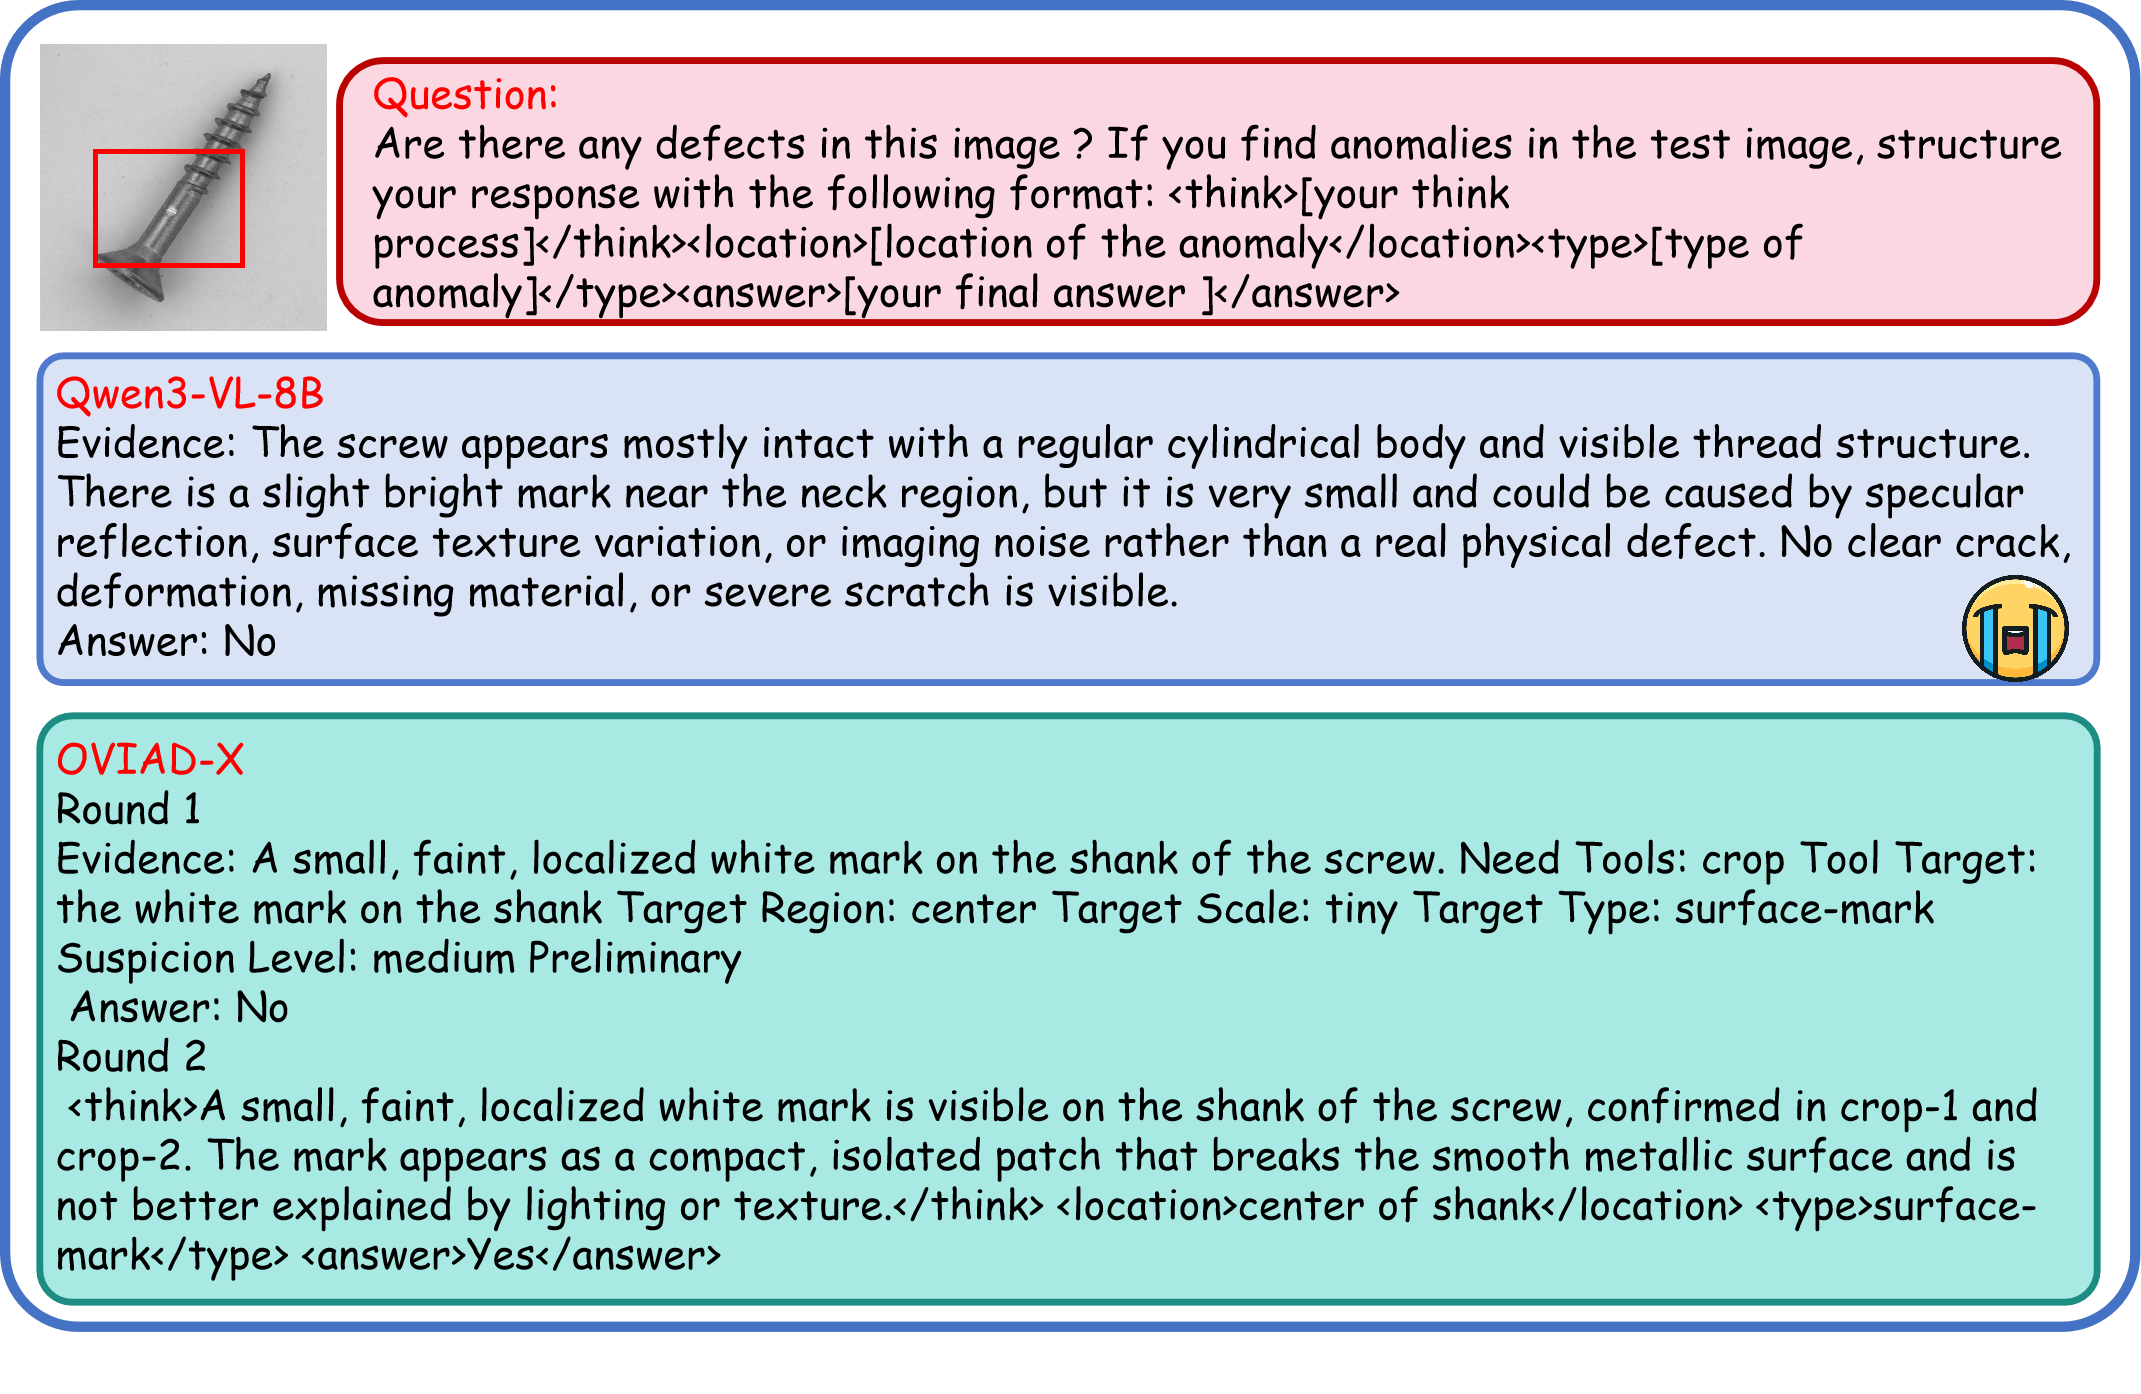
\includegraphics[width=\textwidth]{fig/case3.png }
   \caption{
    Case Study between Qwen3-VL-8B and our method.
    }
  \label{fig:case3}
  \vspace{-1.0em}
\end{figure}

\begin{figure} [h]
  \centering
  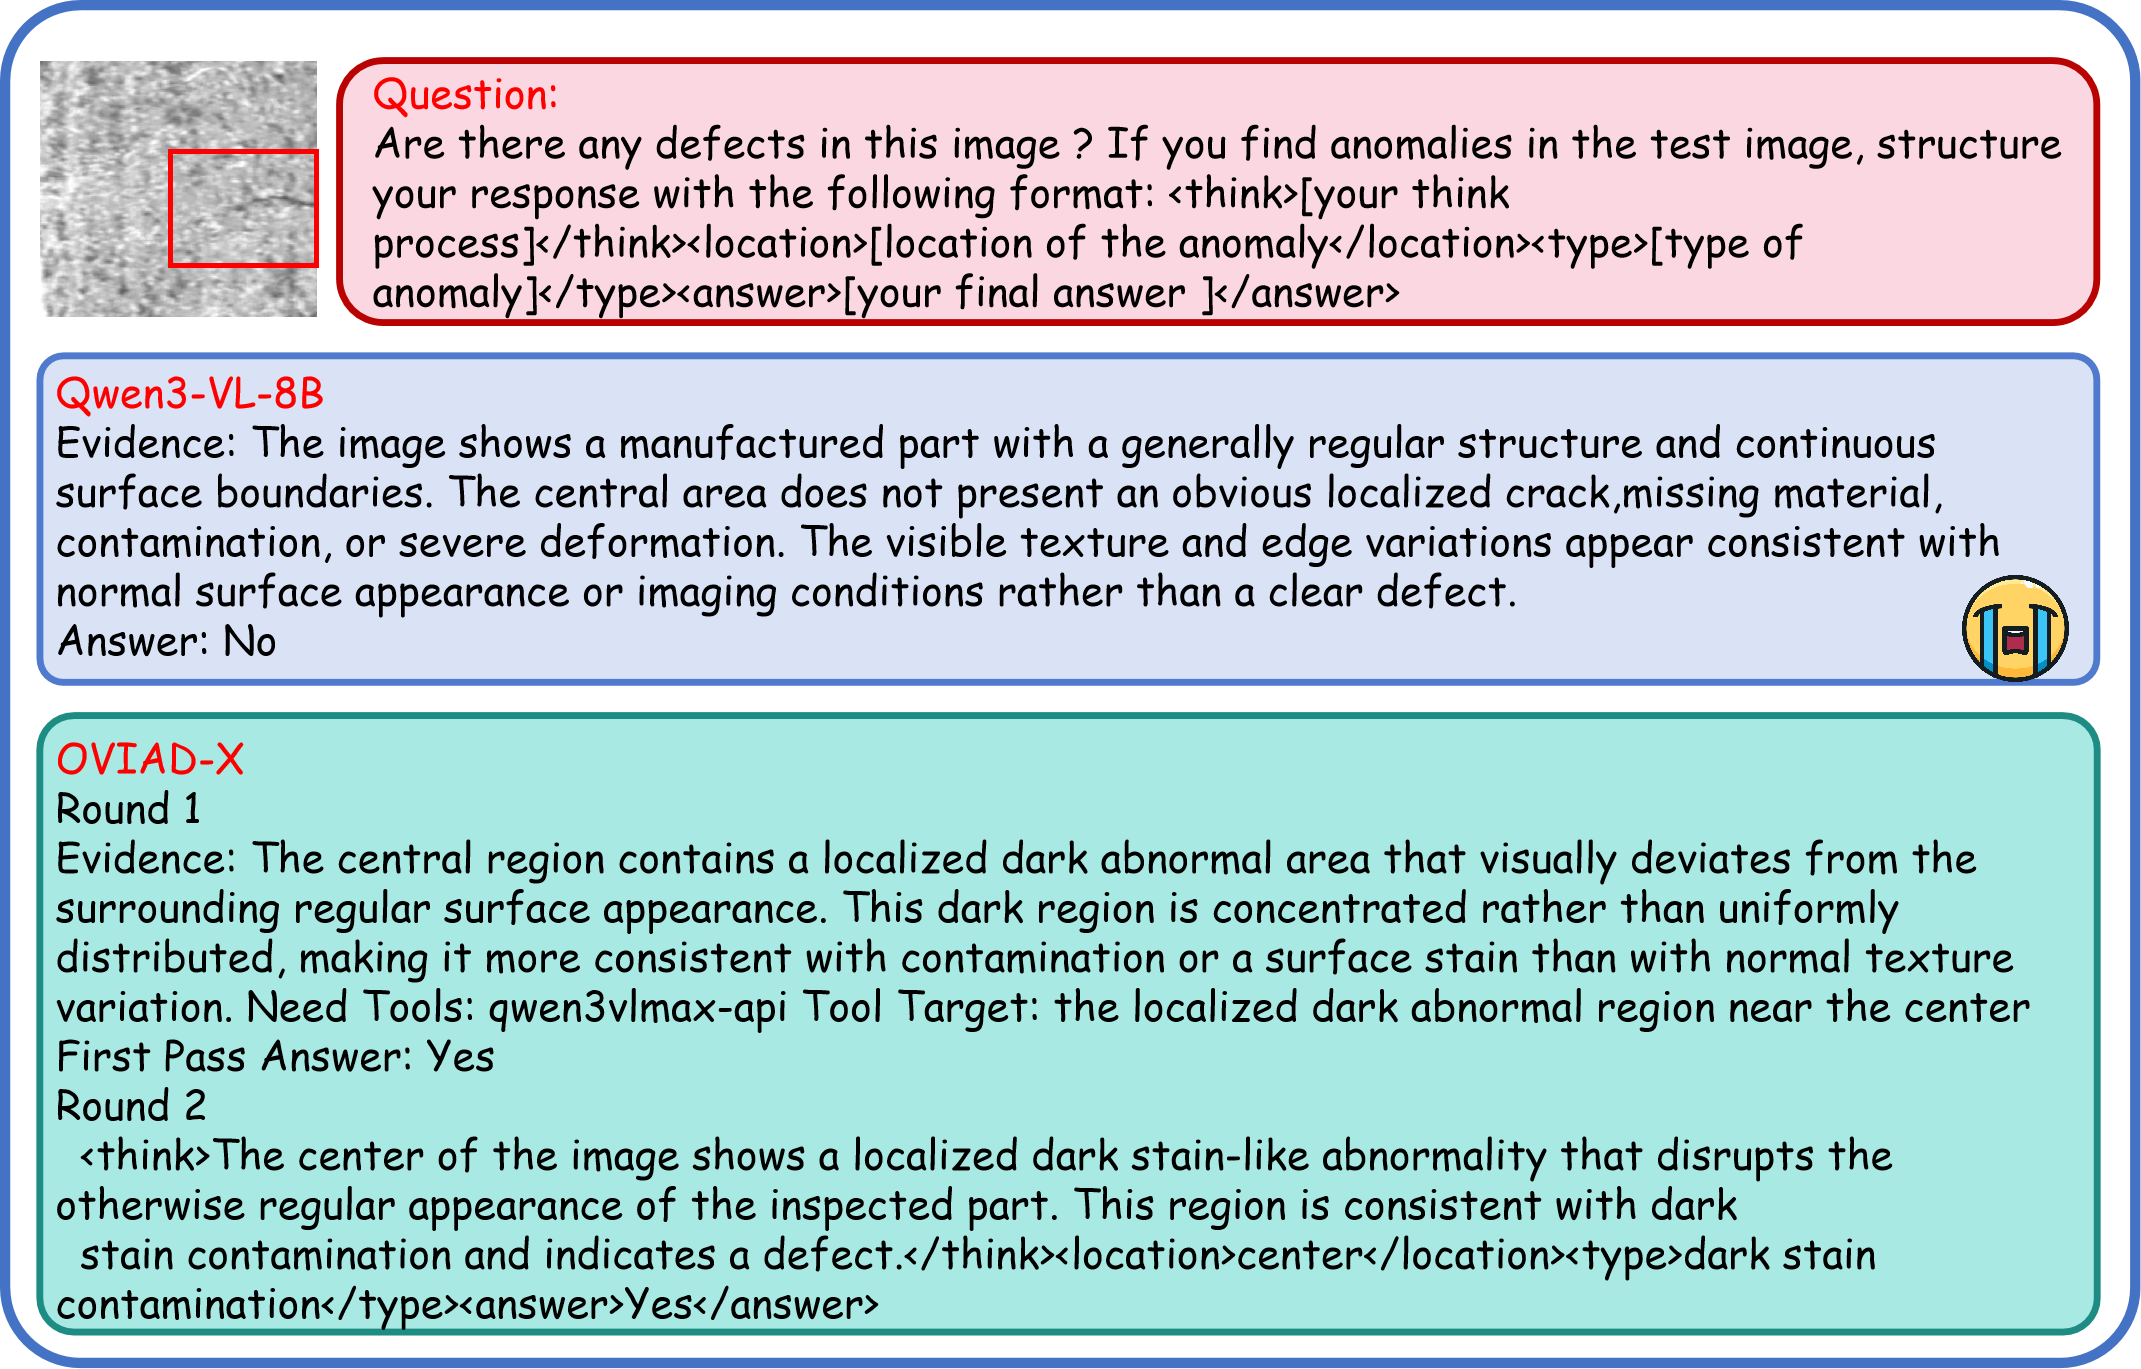
\includegraphics[width=\textwidth]{fig/case2.png }
   \caption{
    Case Study between Qwen3-VL-8B and our method.
    }
  \label{fig:case2}
  \vspace{-1.0em}
\end{figure}

\section{Detailed Related Work}
\label{appx:detailed_related_work}

This section extends the concise related work in the main paper, which discusses three central lines: open-vocabulary industrial anomaly detection, reasoning in multimodal LLMs, and tool-augmented agentic systems. We provide a broader discussion to clarify how IndusAgent is positioned with respect to anomaly detection, multimodal reasoning, knowledge faithfulness, active tool use, vision-language-action models, generative visual modeling, structured representations, and specialized visual perception systems.

\paragraph{Open-vocabulary industrial anomaly detection.}
Industrial anomaly detection has traditionally been studied under closed-set or category-specific assumptions. Reconstruction-based methods learn normal visual patterns and identify anomalies through reconstruction residuals, as represented by autoencoder-based and synthetic-anomaly approaches such as DRAEM and related reconstruction models~\citep{zavrtanik2021draem, bergmann2018improving}. Diffusion-based anomaly detectors further improve generative reconstruction quality, but they may also reconstruct abnormal regions and reduce the separability between normal and defective samples~\citep{wyatt2022anoddpm, mu2023diffusionad}. Feature-embedding methods, including patch-level memory-bank models and probabilistic feature modeling, achieve strong in-distribution performance by comparing local features against normal training distributions~\citep{roth2022patchcore, defard2021padim}, while flow-based methods improve density modeling through invertible transformations~\citep{yu2021fastflow, rudolph2022csflow}. However, these methods usually require category-specific normal data and are therefore less suitable for open-vocabulary inspection. Vision-language approaches such as WinCLIP and AnomalyGPT exploit cross-modal semantic priors to improve zero-shot or few-shot anomaly reasoning~\citep{jeong2023winclip, gu2024anomalygpt}. In contrast to these passive single-pass paradigms, IndusAgent formulates anomaly inspection as an active diagnostic process in which the model can gather local evidence, compare against normalcy priors, and reason over tool feedback.

\paragraph{Multimodal reasoning, knowledge faithfulness, and post-training.}
Recent work on LLM and MLLM reasoning shows that structured intermediate reasoning and post-training can improve task performance beyond direct answer prediction. Chain-of-thought prompting and multimodal reasoning datasets provide the foundation for our Indus-CoT construction~\citep{wei2022chain, zhang2023multimodal}. Reinforcement-learning-based reasoning paradigms, including OpenAI-o1 and DeepSeek-R1, demonstrate that post-training can strengthen deliberative reasoning and self-verification~\citep{jaech2024openaio1, deepseekr1}. This direction has been extended to multimodal settings such as mathematical VQA, reasoning segmentation, and video reasoning~\citep{peng2025lmmr1, liu2025seg, feng2025videor1}. Complementary studies analyze the dynamics of reasoning itself, such as CoT-Kinetics for modeling the reasoning process~\citep{Bi2025CoTKineticsAT}, PROGRESSLM for progress-oriented vision-language reasoning~\citep{zhang2026progresslm}, and adaptive test-time scaling for image editing~\citep{ADE_CoT}. 

Another relevant line of work studies how language models balance parametric knowledge, contextual evidence, and factual confidence. Decoding by Contrasting Knowledge improves model confidence on edited facts by contrasting internal and external knowledge sources~\citep{bi2024decoding}. Context-DPO aligns language models toward context-faithful generation, reducing unsupported reliance on parametric memory when contextual evidence is available~\citep{bi2024context}. Parameters vs. Context further investigates fine-grained control over whether models rely on stored parameters or input context~\citep{bi2025parameters}. These works are closely related to our setting because industrial anomaly detection also requires the model to avoid hallucinated structural assumptions and instead ground its final diagnosis in observable image evidence and retrieved normalcy priors.

From the data and optimization perspective, PRISM studies training-free multimodal data selection~\citep{Bi2025PRISMSI}, while RefineX learns to refine pre-training data at scale from expert-guided programs~\citep{bi2025refinex}. EchoRL explores reinforcement learning through rollout echoing~\citep{bi2026echorl}, and rubric-guided reward design promotes exploration across multiple reasoning domains~\citep{bi2025reward}. These studies motivate our design choice of combining structured SFT with an accuracy-gated RL objective: rather than merely encouraging longer reasoning or more frequent tool use, IndusAgent rewards reasoning trajectories only when they improve the final diagnostic outcome.

\paragraph{Tool-augmented and agentic visual systems.}
Tool-augmented agents extend the capability of foundation models by allowing them to call external modules, interact with structured observations, and revise their reasoning based on feedback. Prior works such as Toolformer and AgentTuning show that tool invocation can be learned or optimized for general language agents~\citep{schick2024toolformer, zeng2024agenttuning}. In multimodal settings, LLaVA-Plus, VPD, TACO, PyVision, and MVoT introduce different ways of combining visual reasoning with tool calls, programmatic execution, or multimodal thoughts~\citep{liu2023llavapluslearningusetools, hu2024visual, ma2024taco, zhao2025pyvision, li2025MVoT}. 

Tool-augmented and reinforcement-based reasoning has also appeared in video understanding and evaluation. Video-STAR reinforces open-vocabulary action recognition with tools~\citep{yuan2025video}, while FactGuard studies agentic video misinformation detection through reinforcement learning~\citep{li2026factguard}. FINGER introduces content-aware fine-grained evaluation with reasoning for AI-generated videos~\citep{chen2025finger}, and Video-CoE reinforces video event prediction through chain-of-events reasoning~\citep{su2026video}. These works suggest that tool use and structured reasoning are particularly useful when the target evidence is fine-grained, temporally distributed, or difficult to capture through a single passive visual encoding.

Instruction-aware and design-oriented agentic systems further demonstrate the generality of tool-based multimodal reasoning. InstructHOI shows the value of context-aware instruction following for human-object interaction detection~\citep{luoinstructhoi}, while AnyLayout studies versatile advertising poster layout generation with MLLMs~\citep{anonymous2025anylayout}. Unlike these general-purpose or task-specific agents, IndusAgent focuses on industrial anomaly inspection, where tool calls must be both visually grounded and cost-aware. Our reward design therefore gates tool utility with diagnostic correctness to discourage indiscriminate tool invocation.

\paragraph{Vision-language-action and embodied reasoning.}
A related line of work studies vision-language-action models, where perception, reasoning, and action are integrated into a unified policy. Survey work on pure VLA models summarizes this trend toward direct multimodal action generation~\citep{zhang2025pure}. In autonomous driving, Reasoning-VLA, CoC-VLA, and AutoDrive-R2 explore how reasoning, causality, and self-reflection can improve decision-making in complex dynamic scenes~\citep{zhang2025reasoning, zhang2026coc, yuan2025autodrive}. Pelican-Unified aims to unify understanding, reasoning, imagination, and action in embodied intelligence~\citep{zhang2026pelican}, while physical autoregressive modeling investigates robotic manipulation without action pretraining~\citep{song2025physical}. Open-future task discovery further considers how agents can discover and organize future human-centric tasks~\citep{song2026human}. 

Although industrial anomaly detection does not require physical actuation, it shares the need for sequential decision-making: the model must decide whether to inspect local regions, retrieve priors, enhance texture, or measure geometry before making a final judgment. Related perception modules in autonomous systems, such as online HD map construction and efficient stereo matching, also reflect the importance of structured spatial understanding~\citep{zhang2025mapexpert, zhang2023ehss}. Beyond high-level action reasoning, structured spatial perception is also essential for embodied and industrial visual systems. For example, cross-view tracking for multi-human 3D pose estimation demonstrates how multi-view geometric cues can support accurate and efficient spatial understanding~\citep{chen2020cross}. Although IndusAgent does not perform 3D pose estimation, it shares the same broader motivation of using structured visual evidence, rather than relying solely on global image-level semantics, to improve fine-grained reasoning.

\paragraph{Generative visual modeling, geometry, and robustness.}
Generative models provide useful priors for visual synthesis, editing, and scene understanding. Multi-modal diffusion Mamba studies end-to-end multimodal diffusion modeling~\citep{lu2025end}, while Layout2Scene and Graph2Scene use semantic layouts or interaction-aware graphs to guide 3D scene generation~\citep{chen2025layout2scene, chen2025graph2scene}. Geometry-aware editing and dense geometry estimation explore how image editing can be constrained or interpreted through 3D structure~\citep{wang2026geometry, wang2025editor}. 

In remote sensing, CRS-Diff, AeroGen, Text2Earth, Change-Agent, and decoupled prompt learning for change captioning study generation, object detection, text-driven synthesis, and interactive interpretation under large-scale visual-domain shifts~\citep{tang2024crs, tang2025aerogen, liu2025text2earth, liu2024changeagent, liu2023decoupling}. Robustness of diffusion models is another important issue, as shown by adversarial and backdoor detection for conditional diffusion models and step-vulnerability-guided diffusion attacks~\citep{yu2025dadet, yu2024step}. These works are not industrial anomaly detectors directly, but they are relevant to IndusAgent because subtle defects often require geometry-aware comparison, texture-sensitive enhancement, and robustness against misleading visual artifacts.

\paragraph{Cross-modal retrieval, alignment, and structured representations.}
Cross-modal alignment and retrieval methods provide another perspective on open-vocabulary visual reasoning. DecAlign studies hierarchical cross-modal alignment for decoupled multimodal representation learning~\citep{qian2025decalign}. Composed image retrieval methods such as ConeSep, TEMA, and HABIT investigate how visual and textual modifications can be jointly modeled for robust retrieval under complex user instructions~\citep{ConeSep, TEMA, HABIT}. These methods emphasize the importance of disentangling visual evidence from linguistic intent, which is also crucial for open-vocabulary anomaly inspection where the model must distinguish true defects from benign variations described by language.

Multi-view and graph-based representation learning further shows the benefit of robust structured representations under incomplete or heterogeneous observations. Sampling-enhanced contrastive multi-view clustering and prototype-driven attribute-missing graph clustering study how representations can be learned under long-short range dependencies or missing attributes~\citep{SEC-LSRM, PAGC}. Multi-scale graph learning also provides useful inspiration for structured perception under sparse or incomplete observations. For example, anti-sparse downscaling with multi-scale graph learning studies how graph structures can propagate information across different spatial resolutions~\citep{fan2025multi}. This is conceptually related to industrial inspection, where subtle local defects must be interpreted together with global object structure and multi-scale contextual cues. Vocabulary recommendation for spatiotemporal data discovery also highlights how structured semantic resources can support data interpretation across domains~\citep{cui2019vocabulary}.

\paragraph{Specialized visual perception in scientific, medical, graph, and wearable domains.}
Several related works address robust perception under domain-specific noise, limited labels, or specialized sensors. In scientific and medical imaging, self-supervised cryo-electron tomography restoration, pathology foundation-model fusion, adaptive label correction for noisy medical segmentation, self-supervised neuron segmentation with multi-agent reinforcement learning, and evolutionary medical prompt optimization all study how to improve reliability in high-stakes visual analysis settings~\citep{Yang_2021_ICCV, yang2025fusionmultiscaleheterogeneouspathology, qian2025adaptive, chen2023self, chen2026empower}. Wearable sensing systems such as KineticsSense and PPGSpeech further demonstrate the broader role of multimodal sensor fusion for fine-grained perception and inference~\citep{10.1145/3749462, 11271667}. 

In graph learning, self-purified masked graph autoencoders, robustness-aware masking strategies, and adversarially robust graph prompt tuning study how representation learning systems can remain stable under noise or attacks~\citep{song2025spmgae, song2025equipping, song2025gpromptshield}. Although these works target different domains, they share with IndusAgent the central motivation of making model predictions more robust by incorporating structured priors, external feedback, or robustness-aware training objectives. Finally, hierarchical spatiotemporal reward modeling for video further supports the broader trend of using structured reward signals to align multimodal models with complex perceptual judgments~\citep{wang2026cac}.
  
\section{Limitations}
\label{sec:limitations}

Despite its promising performance, IndusAgent still has several limitations. First, the active inspection process introduces additional inference overhead compared with single-pass MLLM inference, since external tools such as cropping, enhancement, and prior retrieval require extra computation. Second, the framework depends on the reliability of tool feedback; inaccurate crops, noisy enhanced maps, or incomplete normalcy priors may mislead the agent and affect the final diagnosis. Third, our current experiments mainly focus on image-level anomaly judgment, while more fine-grained evaluations, such as pixel-level localization, region-level grounding, and tool-use efficiency analysis, are needed to better understand the agent's diagnostic behavior. Finally, Indus-CoT is generated with the assistance of a strong teacher model and rule-based validation, which may introduce teacher or prompt-template bias. Future work will explore more efficient tool-use policies, stronger tool robustness, and more diverse expert supervision for practical industrial deployment.




\newpage

\input{checklist.tex}










\end{document}